%Preâmbulo
\documentclass[12pt, a4paper]{article}
\usepackage[brazilian]{babel}
\usepackage[utf8]{inputenc}
%\usepackage[left=2cm,right=2cm,top=2cm,bottom=2cm]{geometry}
\usepackage{indentfirst}

\usepackage{amsmath, amsfonts, amssymb}
\DeclareMathOperator{\sen}{sen}
\DeclareMathOperator{\tg}{tg}
\DeclareMathOperator{\cossec}{cossec}
\DeclareMathOperator{\arcsen}{arcsen}
\DeclareMathOperator{\arctg}{arctg}
\DeclareMathOperator{\arccossec}{arccossec}
\DeclareMathOperator{\e}{e}
\newcommand{\limite}{\displaystyle\lim}
\newcommand{\integral}{\displaystyle\int}
\newcommand{\iintegral}{\displaystyle\iint}
\usepackage[normalem]{ulem}
\newcommand{\overstrike}[1]{\ifmmode\text{\sout{\ensuremath{#1}}}\else\sout{#1}\fi}

\usepackage{graphicx}
\graphicspath{{img/}}
\usepackage{float}

\title{Curso de integrais duplas e triplas}
\author{César Antônio de Magalhães \\ ceanma@gmail.com}
\date{\today}

%Corpo do texto
\begin{document}
	\maketitle\newpage
	
	\tableofcontents\newpage
	
	%\listoftables\newpage
	
	\listoffigures\newpage
	
	%\begin{abstract}	
	%\end{abstract}
	
	\part{Integrais duplas}	
		\section{Invertendo os limites de integração - Aula 1}			
			\begin{enumerate}
	\item Exercício
	
	\begin{figure}[H]
		\caption{Integrais duplas - Aula 1 - Exercício I e II}
		\label{v01_a01_e01}
		\centering
		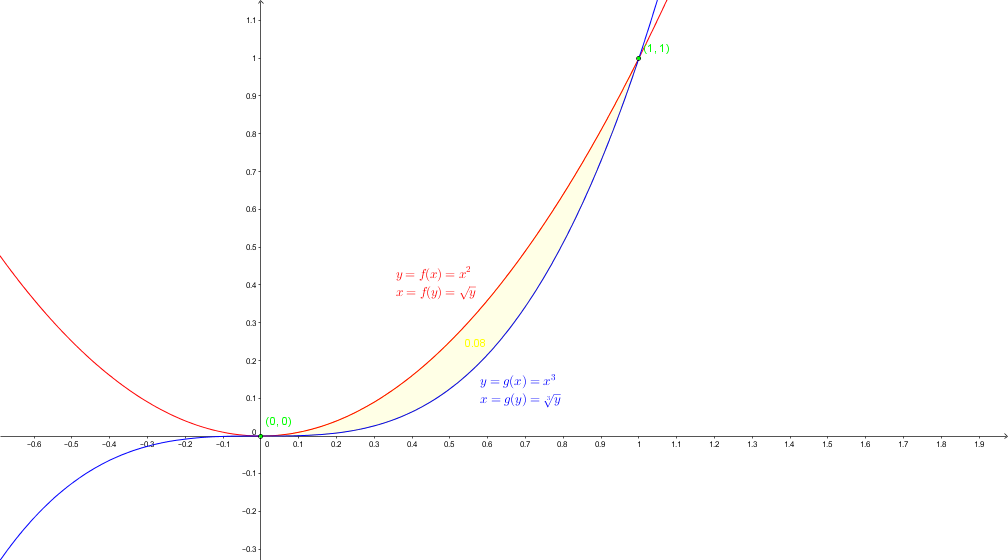
\includegraphics[width=\textwidth]{v01_a01_e01.png}		
	\end{figure}
				
	$f(x) = x^2;\; g(x) = x^3$\newline
	$x = 0 \Rightarrow f(0) = g(0) \Rightarrow 0^2 = 0^3$\newline
	$x = 1 \Rightarrow f(1) = g(1) \Rightarrow 1^2 = 1^3$\newline
	
	$a = \integral_0^1 dx \integral_{g(x)}^{f(x)} dy = \integral_0^1 dx \integral_{x^3}^{x^2} dy = \integral_0^1 dx\, [y]_{x^3}^{x^2} = \integral_0^1 dx \left[x^2 - x^3\right] = \integral_0^1 x^2\, dx - \integral_0^1 x^3\, dx = \left[\dfrac{x^3}{3} - \dfrac{x^4}{4}\right]_0^1 = \left[\dfrac{4x^3 - 3x^2}{12}\right]_0^1 = \dfrac{1}{12}\left[4x^3 - 3x^2\right]_0^1 = \dfrac{1}{12}\left[x^2\left(4x - 3\right)\right]_0^1 = \dfrac{1}{12}\left[1^2\left(4 \cdot 1 - 3\right) \overstrike{- 0^2\left(4 \cdot 0 - 3\right)}\right] = \dfrac{1}{12} = 0,08\overline{3}$
					
	\item Exercício
	
	$f(x) = x^2 \Rightarrow f(y) = \sqrt{y};\; g(x) = x^3 \Rightarrow g(y) = \sqrt[3]{y}$\newline
	$y = 0 \Rightarrow f(0) = g(0) \Rightarrow \sqrt{0} = \sqrt[3]{0}$\newline
	$y = 1 \Rightarrow f(1) = g(1) \Rightarrow \sqrt{1} = \sqrt[3]{1}$\newline
	
	$a = \integral_0^1 dy \integral_{f(y)}^{g(y)} dx = \integral_0^1 dy \integral_{\sqrt{y}}^{\sqrt[3]{y}} dx = \integral_0^1 dy\, [x]_{\sqrt{y}}^{\sqrt[3]{y}} = 
	\integral_0^1 dy \left[\sqrt[3]{y} - \sqrt{y}\right] = \integral_0^1 \sqrt[3]{y}\, dy - \integral_0^1 \sqrt{y}\, dy = \integral_0^1 y^{\frac{1}{3}}\, dy - \integral_0^1 y^{\frac{1}{2}}\, dy = \left[\dfrac{y^{\frac{4}{3}}}{\left(\dfrac{4}{3}\right)} - \dfrac{y^{\frac{3}{2}}}{\left(\dfrac{3}{2}\right)}\right]_0^1 = \left[\dfrac{3 \sqrt[3]{y^4}}{4} - \dfrac{2 \sqrt{y^3}}{3}\right]_0^1 = \left[\dfrac{9 \sqrt[3]{y^4} - 8 \sqrt{y^3}}{12}\right]_0^1 = \dfrac{1}{12}\left[9 \sqrt[3]{y^4} - 8 \sqrt{y^3}\right]_0^1 =\\ \dfrac{1}{12}\left[\left(9 \sqrt[3]{1^4} - 8 \sqrt{1^3}\right) \overstrike{-\left(9 \sqrt[3]{0^4} - 8 \sqrt{0^3}\right)}\right] = \dfrac{1}{12}(9 - 8) = \dfrac{1}{12} = 0,08\overline{3}$
\end{enumerate}		
		\section{Determinação da região de integração - Aula 2}		
			\begin{enumerate}
	\item Exercício
	
	$R = \left\{(x, y) \in \mathbb{R}^2 \,|\, 0 \leq x \leq 2 \,,\, 0 \leq y \leq 6 \right\}$
	
	\begin{figure}[H]
		\caption{Integrais duplas - Aula 2 - Exercício I}
		\label{v02_a02_e01}
		\centering
		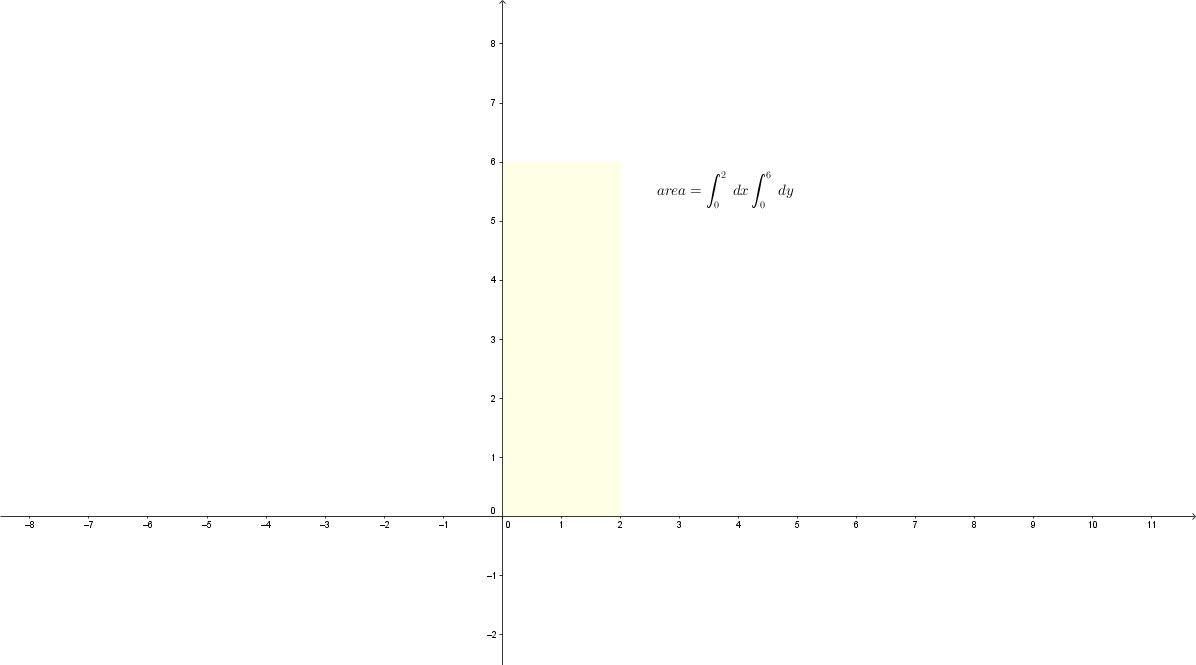
\includegraphics[width=\textwidth]{v02_a02_e01.png}		
	\end{figure}
	
	$a = \integral_0^2 dx \integral_0^6 dy = \integral_0^2 dx\, [y]_0^6 = \integral_0^2 dx\, [6 - 0] = 6\integral_0^2 dx = 6[x]_0^2 = 6[2 - 0] = 6 \cdot 2 = 12$
	
	\item Exercício
	
	$R = \left\{(x, y) \in \mathbb{R}^2 \,|\, 0 \leq x \leq 1 \,,\, x \leq y \leq 2x \right\}$
						
	\begin{figure}[H]
		\caption{Integrais duplas - Aula 2 - Exercício II}
		\label{v02_a02_e02}
		\centering
		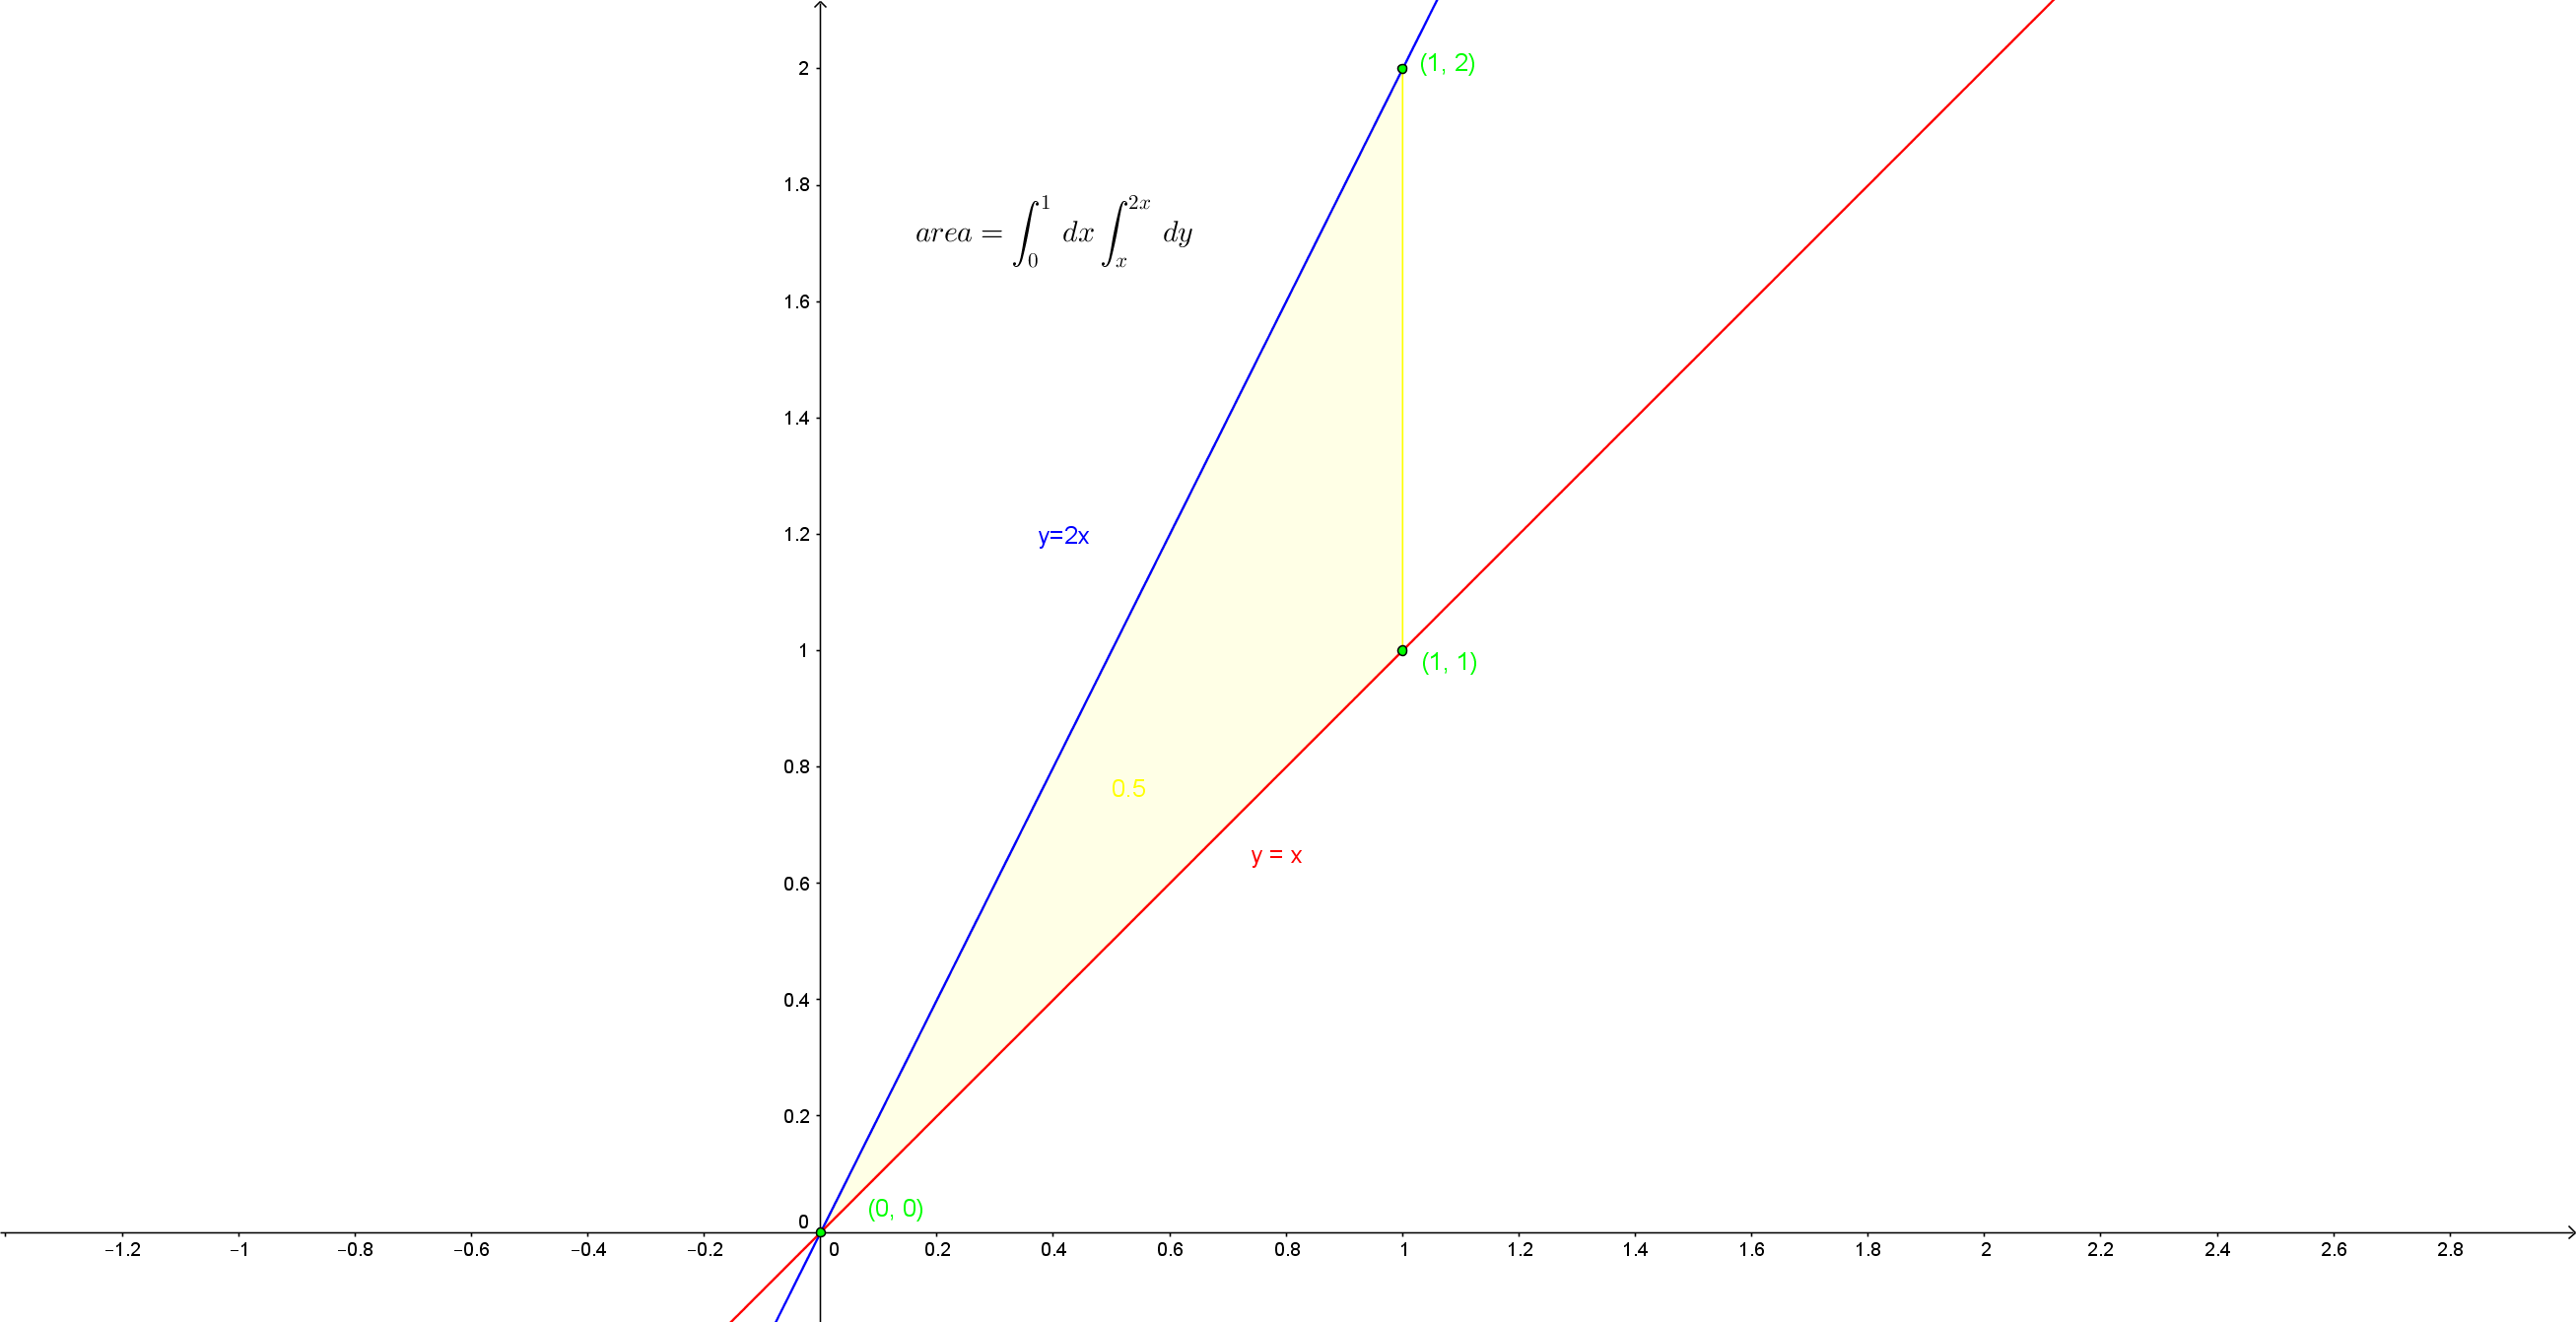
\includegraphics[width=\textwidth]{v02_a02_e02.png}		
	\end{figure}
	
	$a = \integral_0^1 dx \integral_{x}^{2x} dy = \integral_0^1 dx\, [y]_{x}^{2x} = \integral_0^1 dx\, [2x - x] = 2\integral_0^1 x\, dx - \integral_0^1 x\, dx = \left[\overstrike{2}\dfrac{x^2}{\overstrike{2}} - \dfrac{x^2}{2}\right]_0^1 = \left[\dfrac{2x^2 - x^2}{2}\right]_0^1 = \dfrac{1}{2}\left[x^2\right]_0^1 = \dfrac{1}{2}\left[1^2 \overstrike{- 0^2}\right] = \dfrac{1}{2} = 0,5 $
	
	\item Exercício
	
	$R = \left\{(x, y) \in \mathbb{R}^2 \,|\, 0 \leq y \leq 1 \,,\, 0 \leq x \leq \sqrt{1 - y^2} \right\}$
	
	$y = 0,\, y=1$\newline
	$x = 0,\, x = \sqrt{1 - y^2} \Rightarrow x^2 = 1 - y^2 \Rightarrow x^2 - 1 = -y^2 \Rightarrow y^2 = -x^2 + 1 \Rightarrow y = \sqrt{1 -x^2}$
					
	\begin{figure}[H]
		\caption{Integrais duplas - Aula 2 - Exercício III}
		\label{v02_a02_e03}
		\centering
		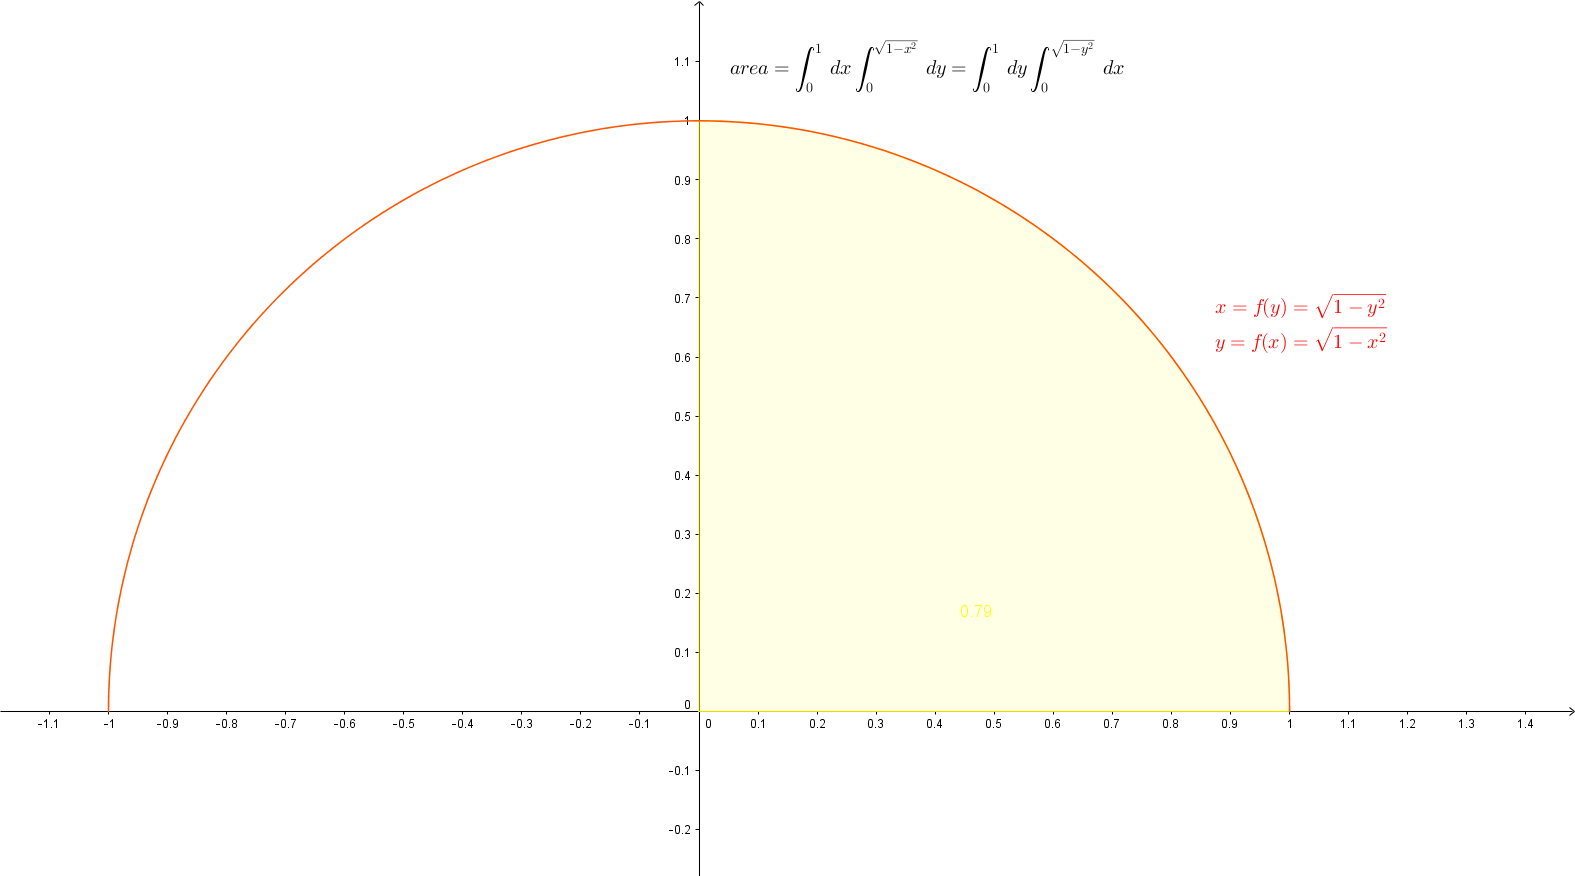
\includegraphics[width=\textwidth]{v02_a02_e03.png}		
	\end{figure}
	
	$a = \integral_0^1 dy \integral_0^{f(y)} dx = \integral_0^1 dy \integral_0^{\sqrt{1 - y^2}} dx = \integral_0^1 dy\, [x]_0^{\sqrt{1 - y^2}} = \integral_0^1 dy\, \left[\sqrt{1 - y^2} - 0\right] = \integral_0^1 \sqrt{1 - y^2}\, dy = \integral_0^1 \sqrt{1 - \sen^2(t)}\, \cos(t) dt = \integral_0^1 \sqrt{\cos^2(t)}\, \cos(t) dt = \integral_0^1 \cos(t)\cos(t) dt = \integral_0^1 \cos^2(t) dt = \integral_0^1 \dfrac{1 + \cos(2t)}{2} dt = \dfrac{1}{2}\integral_0^1 \left[1 + \cos(2t)\right] dt = \dfrac{1}{2}\integral_0^1 dt + \dfrac{1}{2}\integral_0^1 \cos(2t) dt = \dfrac{1}{2}\integral_0^1 dt + \dfrac{1}{2}\integral_0^1 \cos(u) \dfrac{du}{2} = \dfrac{1}{2}\integral_0^1 dt + \dfrac{1}{4}\integral_0^1 \cos(u)\, du = \left[\dfrac{1}{2}t + \dfrac{1}{4}\sen(u)\right]_0^1 = \left[\dfrac{t}{2} + \dfrac{\sen(2t)}{4}\right]_0^1 = \left[\dfrac{t}{2} + \dfrac{2\sen(t)\cos(t)}{4}\right]_0^1 = \left[\dfrac{t + \sen(t)\cos(t)}{2}\right]_0^1 = \dfrac{1}{2}\left[\arcsen(y) + y\sqrt{1 - y^2}\right]_0^1 =\\ \dfrac{1}{2}\left[\left(\arcsen(1) \overstrike{+ 1 \cdot\sqrt{1 - 1^2}}\right) - \left(\arcsen(0) \overstrike{+ 0 \cdot \sqrt{1 - 0^2}}\right)\right] = \dfrac{1}{2}\left[\dfrac{\pi}{2} - 0\right] = \dfrac{\pi}{4} = 0,785$ \newline\newline
	$y = \sen(t) \Rightarrow dy = \cos(t) dt$\newline
	$u = 2t \Rightarrow \dfrac{du}{2} = dt$\newline\newline
	$\sen(t) = \dfrac{co}{h} = \dfrac{y}{1} = y$\newline
	$h^2 = co^2 + ca^2 \Rightarrow 1 = y^2 + ca^2 \Rightarrow ca = \sqrt{1 - y^2}$\newline
	$\cos(t) = \dfrac{ca}{h} = \dfrac{\sqrt{1 - y^2}}{1} = \sqrt{1 - y^2}$\newline
	$y = \sen(t) \Rightarrow t = \arcsen(y)$
	
	\item Exercício
	
	$y = x^2 + 1 ,\, y = -x^2 - 1 ;\; x = 1 ,\, x = -1$\newline
	$R = \left\{(x, y) \in \mathbb{R}^2 \,|\, -1 \leq x \leq 1 \,,\, -x^2 - 1 \leq y \leq x^2 + 1 \right\}$
	
	\begin{figure}[H]
		\caption{Integrais duplas - Aula 2 - Exercício IV}
		\label{v02_a02_e04}
		\centering
		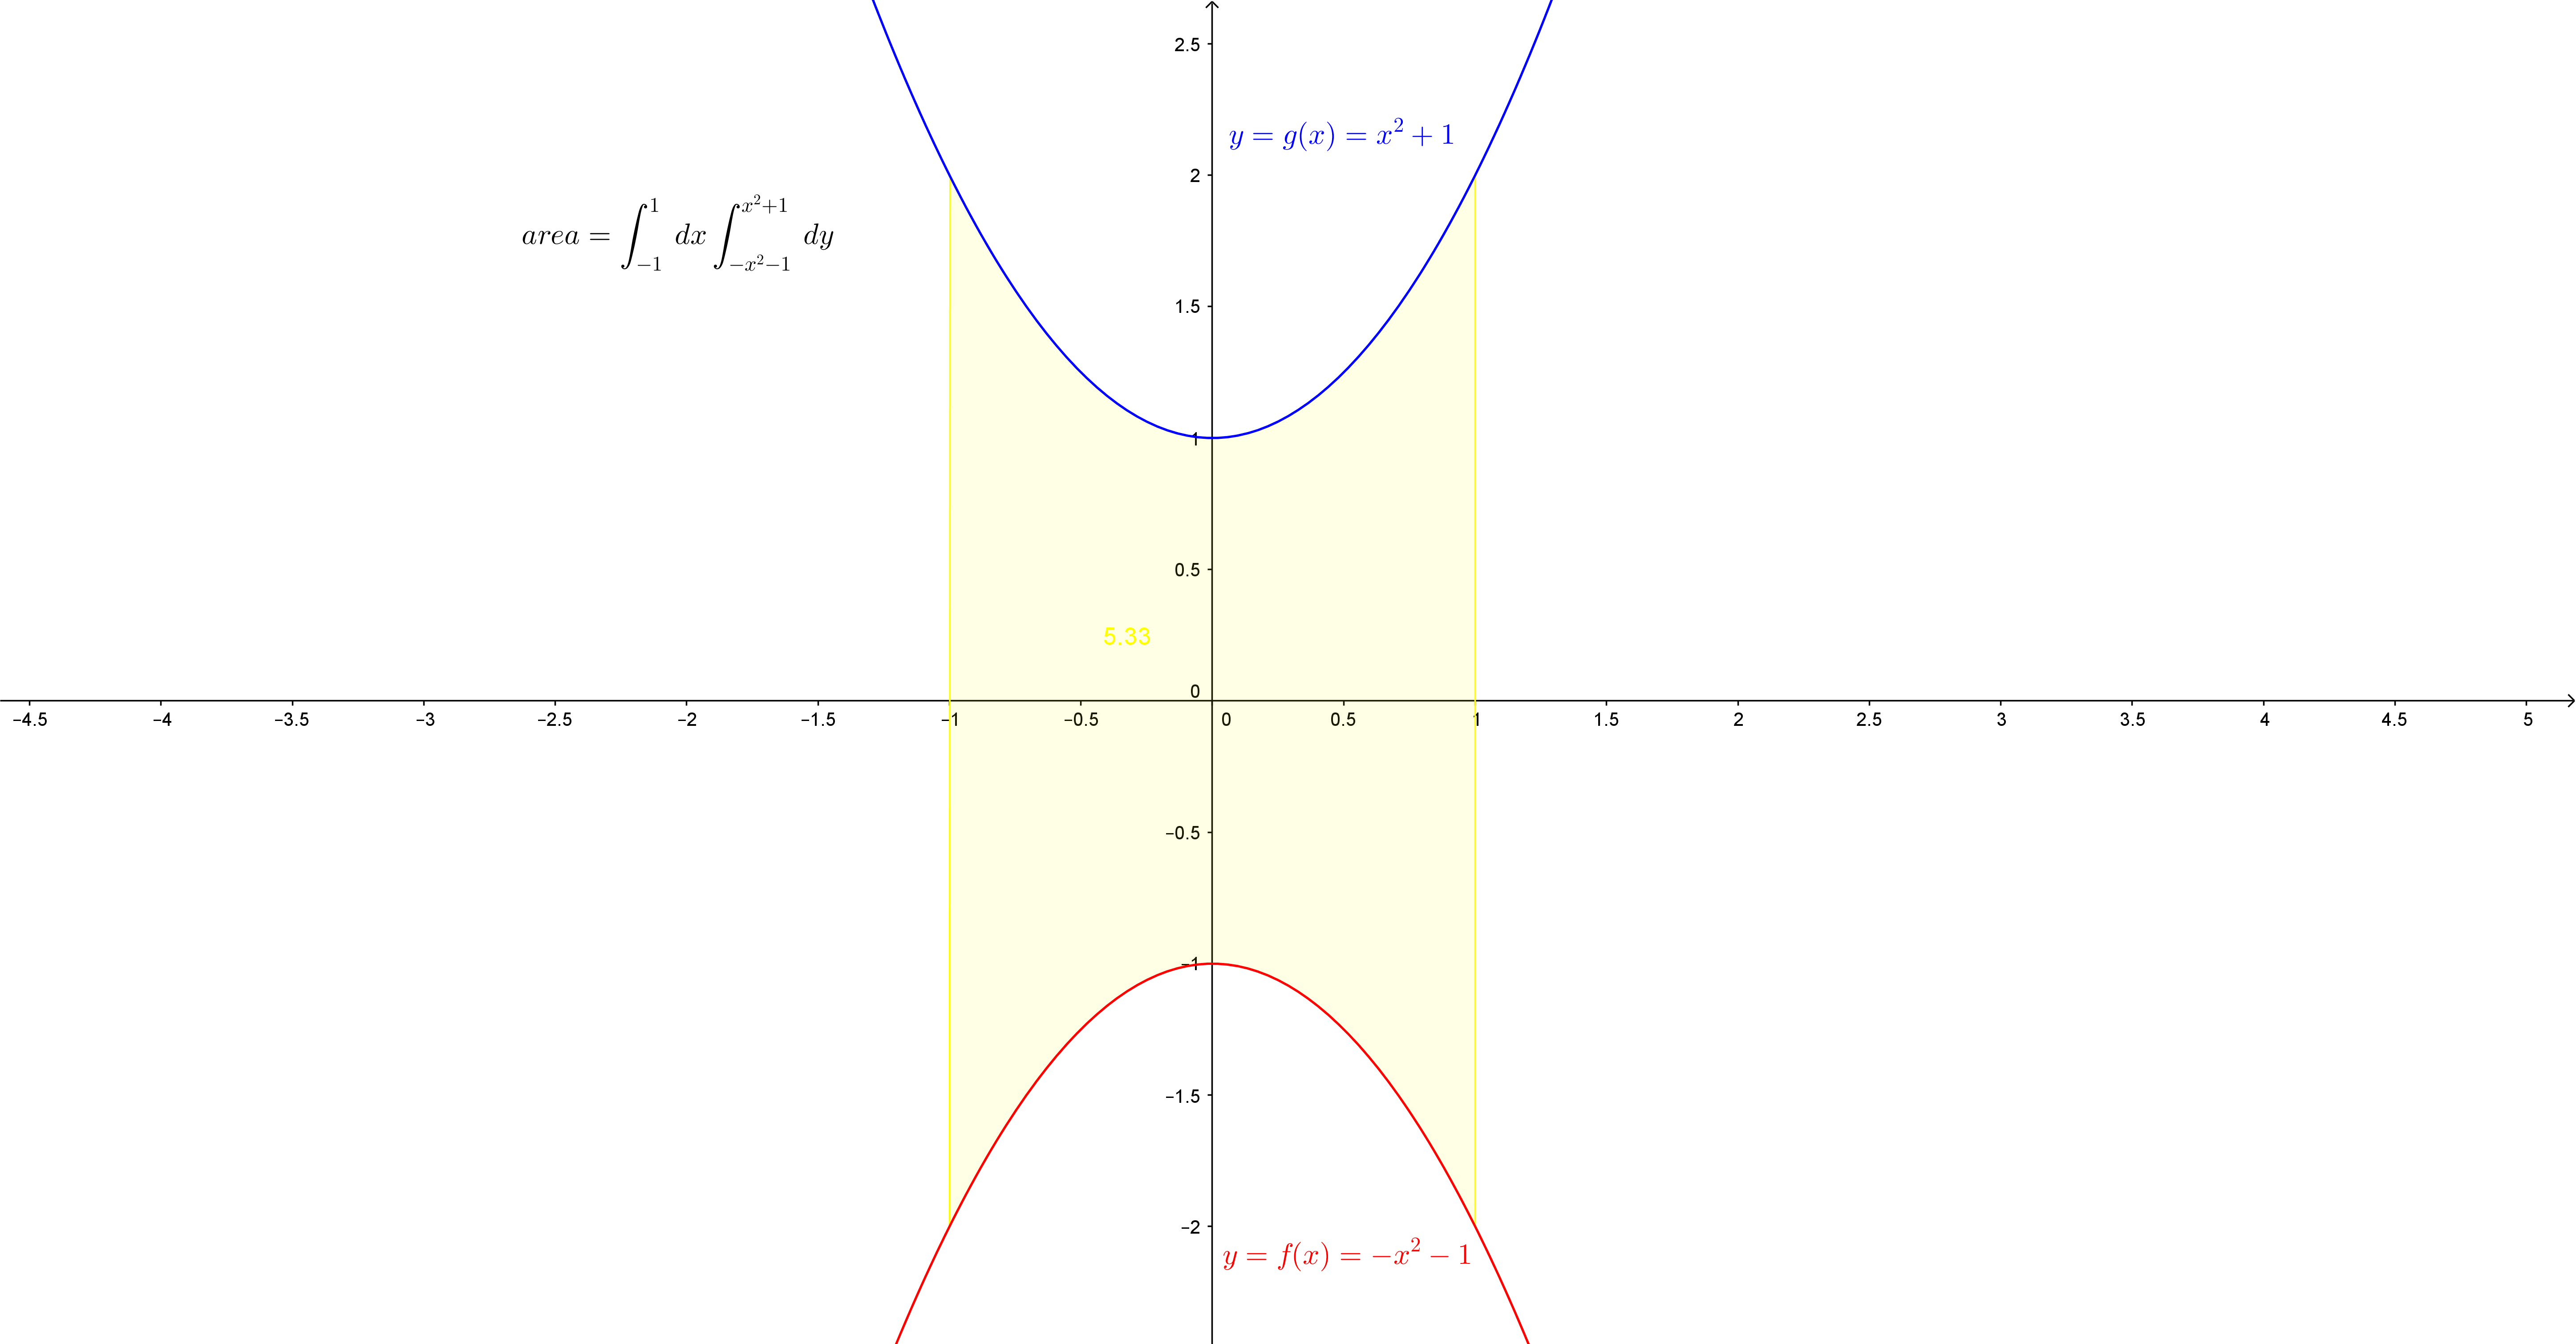
\includegraphics[width=\textwidth]{v02_a02_e04.png}		
	\end{figure}
	
	$a = \integral_{-1}^1 dx \integral_{f(x)}^{g(x)} dy = \integral_{-1}^1 dx \integral_{-x^2 - 1}^{x^2 + 1} dy = \integral_{-1}^1 dx\, [y]_{-x^2 - 1}^{x^2 + 1} = \integral_{-1}^1 dx\, \left[x^2 + 1 - \left(-x^2 - 1\right)\right] = \integral_{-1}^1 dx\, \left[x^2 + 1 + x^2 + 1\right] = \integral_{-1}^1 dx\, \left[2x^2 + 2\right] = 2\integral_{-1}^1 x^2\, dx + 2\integral_{-1}^1 dx = \left[2\dfrac{x^3}{3} +  2x\right]_{-1}^1 = \left[2\left(\dfrac{x^3 + 3x}{3}\right)\right]_{-1}^1 = \dfrac{2}{3}\left[x\left(x^2 + 3\right)\right]_{-1}^1 = \\ \dfrac{2}{3}\left[1 \cdot \left(1^2 + 3\right) - (-1)\left((-1)^2 + 3\right)\right] = \dfrac{2}{3}(4 + 4) = \dfrac{2}{3}8 = \dfrac{16}{3} = 5,\overline{3}$
	
	\item Exercício
	
	$R = \left\{(x, y) \in \mathbb{R}^2 \,|\, 0 \leq y \leq 2 \,,\, -y \leq x \leq y \right\}$
	
	\begin{figure}[H]
		\caption{Integrais duplas - Aula 2 - Exercício V}
		\label{v02_a02_e05}
		\centering
		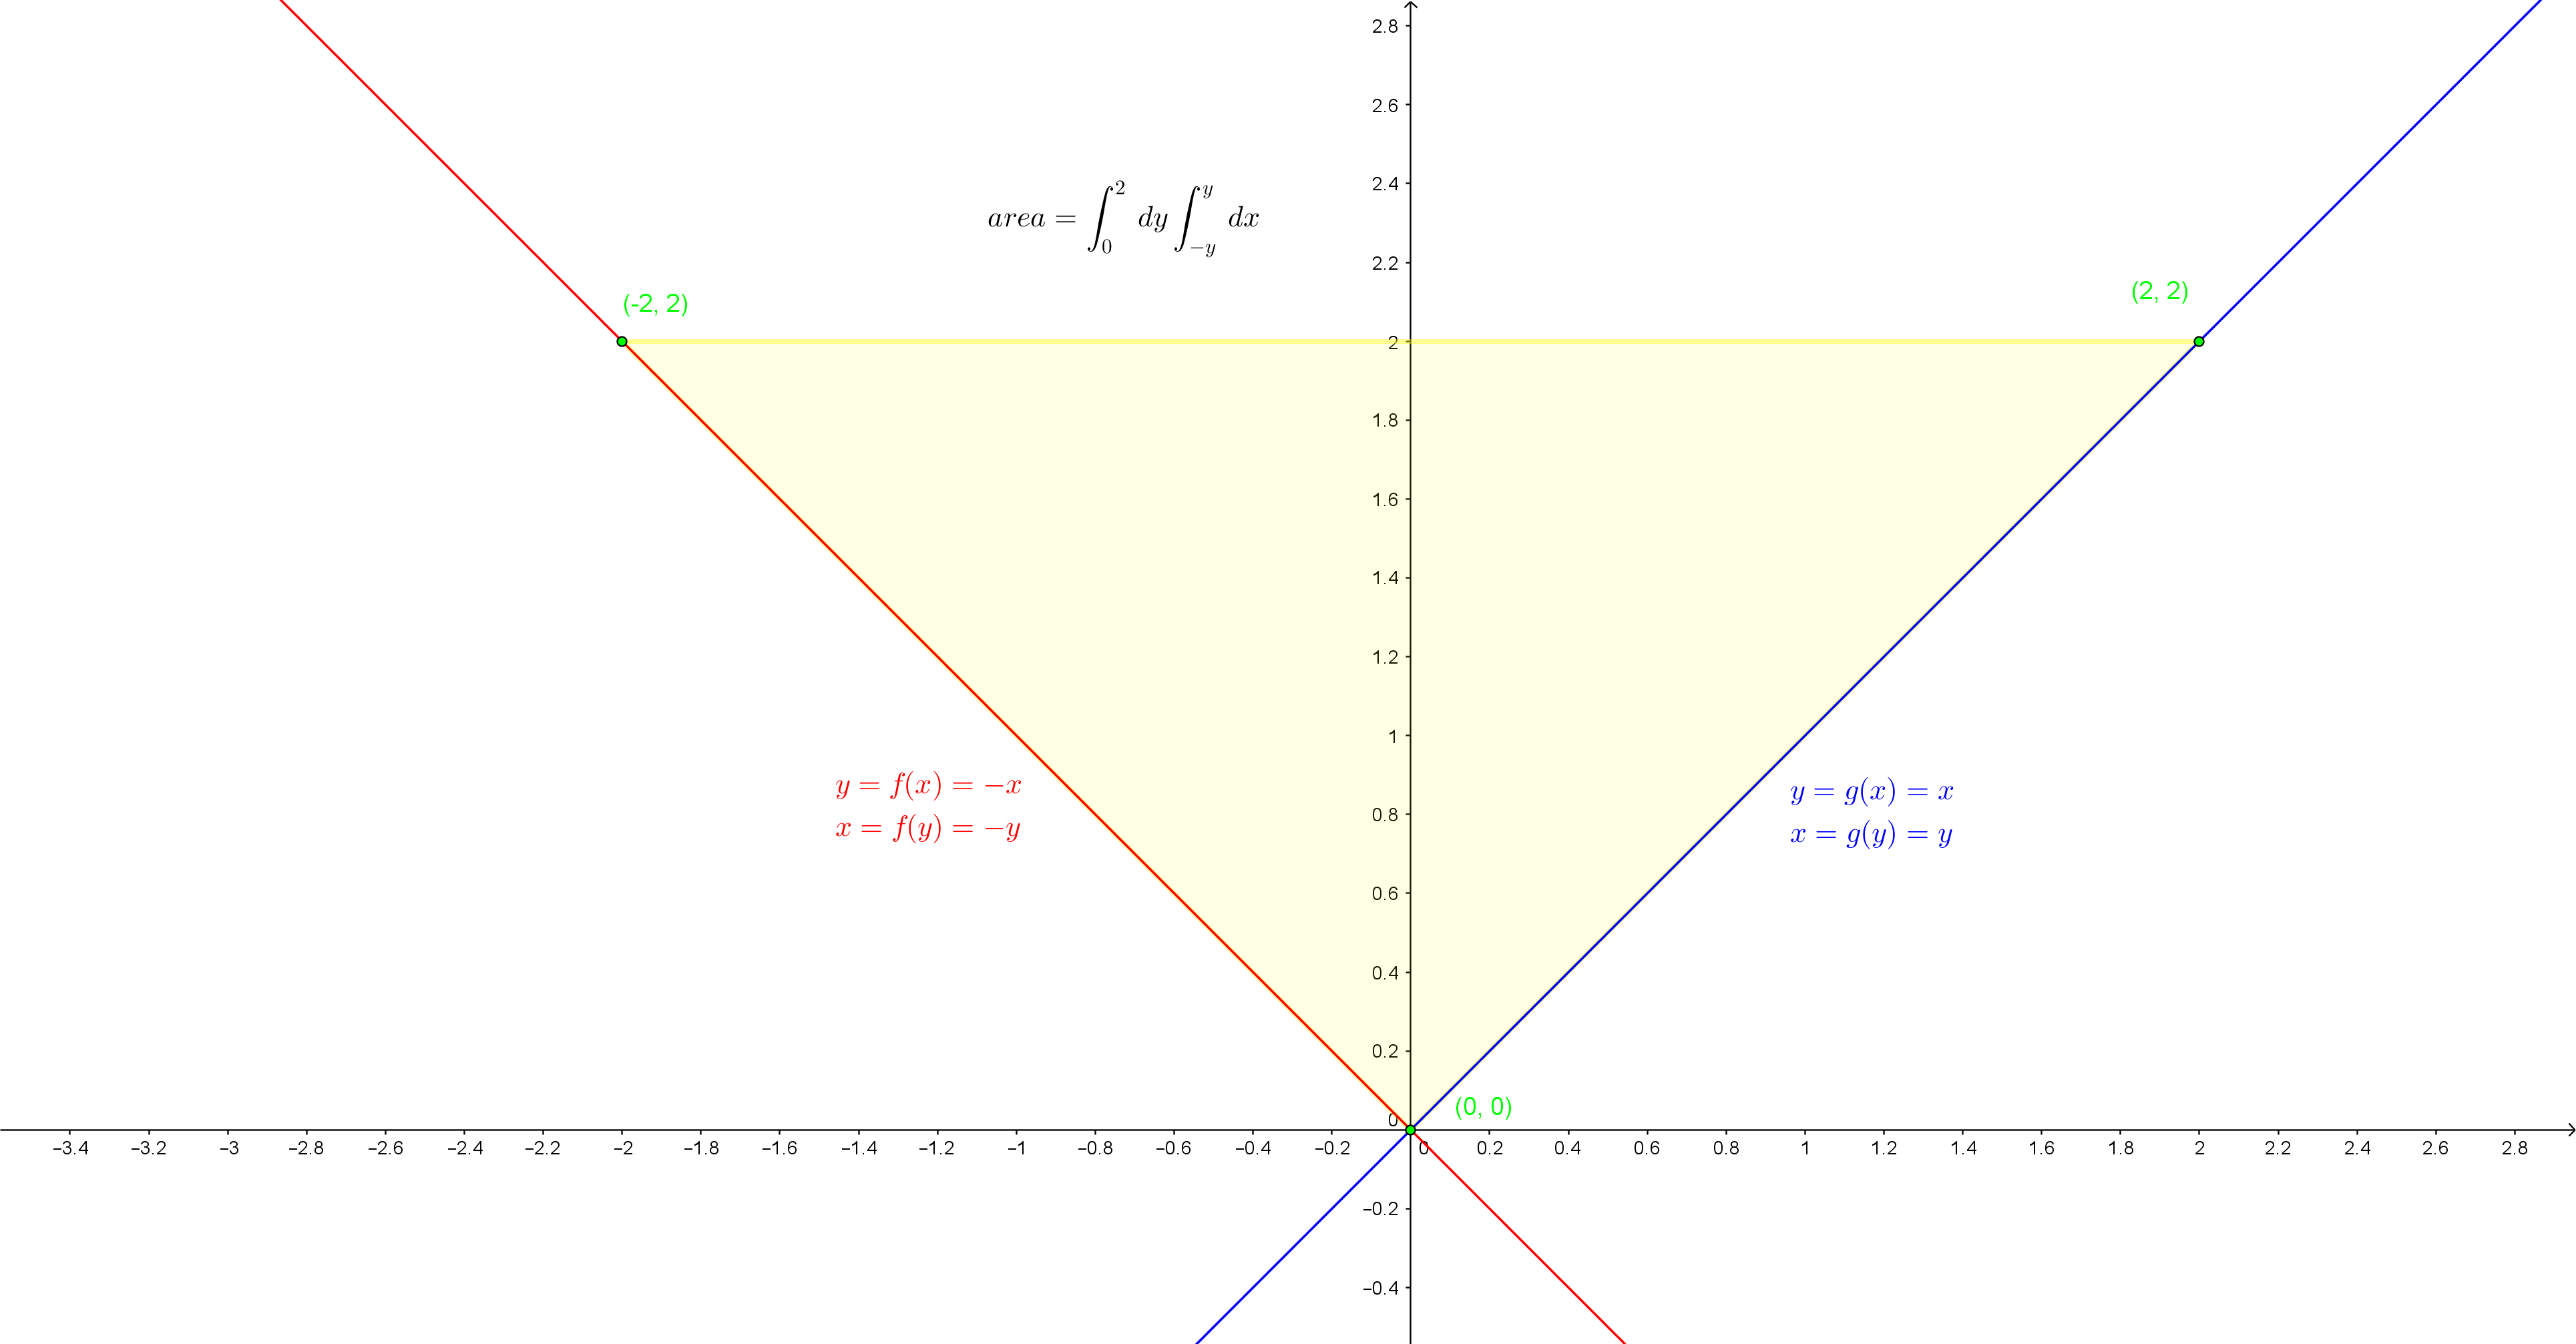
\includegraphics[width=\textwidth]{v02_a02_e05.png}		
	\end{figure}
	
	$a = \integral_0^2 dy \integral_{f(y)}^{g(y)} dx = \integral_0^2 dy \integral_{-y}^y dx = \integral_0^2 dy\, [x]_{-y}^y = \integral_0^2 dy\, [y - (-y)] = \integral_0^2 dy\, [2y] = 2\integral_0^2 y\, dy = \left[\overstrike{2}\frac{y^2}{\overstrike{2}}\right]_0^2 = 2^2 - 0^2 = 4$	
\end{enumerate}		
		\section{Cálculo de volume - Aula 3}
			\begin{enumerate}
	\item Exercício
	
	\begin{figure}[H]
		\centering
		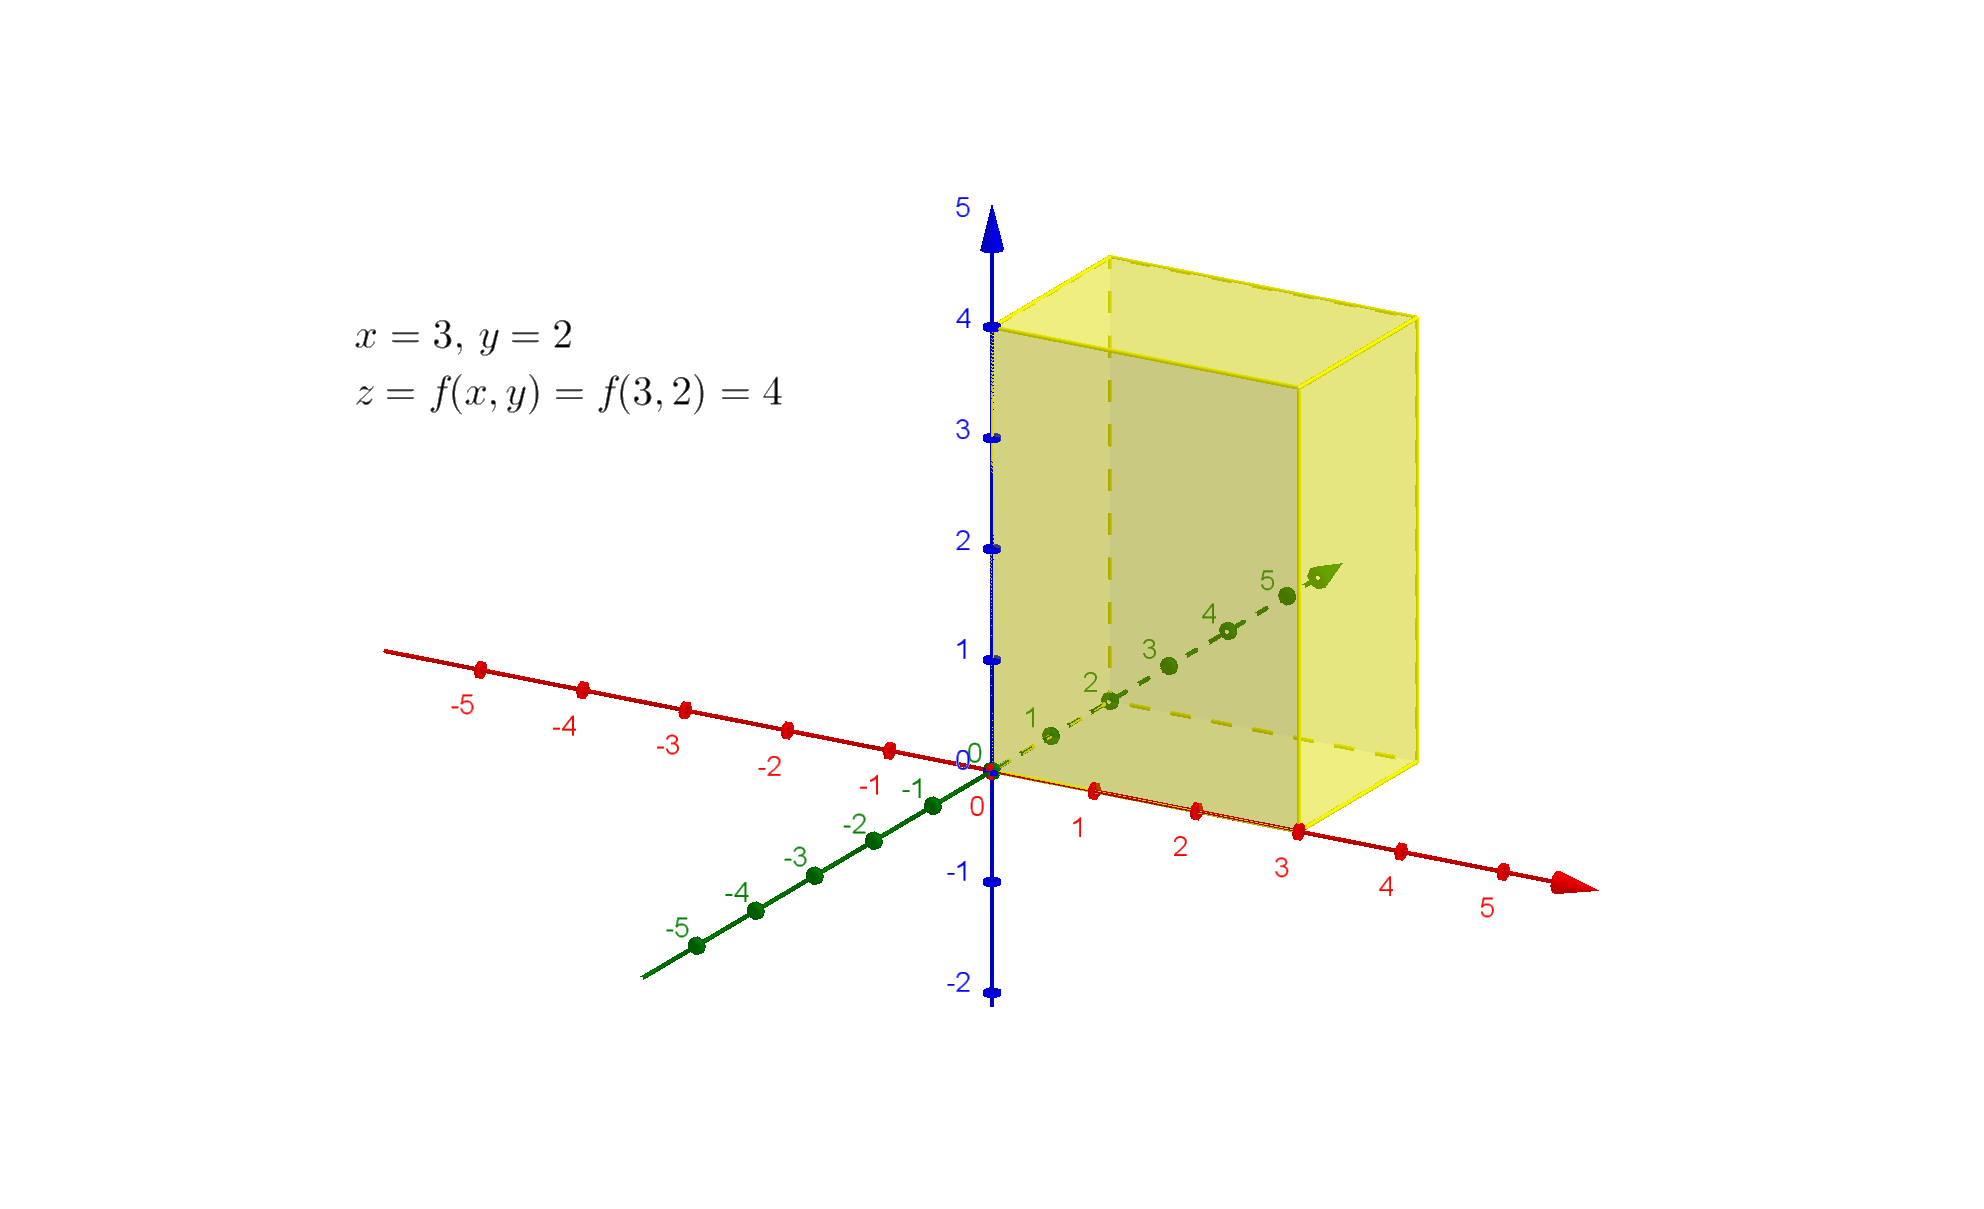
\includegraphics[width=\textwidth]{v01_a03_e01.png}
		\caption{Integrais duplas - Aula 3 - Exercício I}
		\label{v01_a03_e01}
	\end{figure}
	
	$z = 4;\; dz = dx dy$\newline\newline
	$v = \integral_0^3 \integral_0^2 z\, dz = \integral_0^3 \integral_0^2 4\, dy dx = 4\integral_0^3 dx \integral_0^2 dy = 4\integral_0^3 dx\, [y]_0^2 = 4\integral_0^3 dx\, [2 - 0] = 8\integral_0^3 dx = 8[x]_0^3 = 8[3 - 0] = 8 \cdot 3 = 24$\newline
	
	\item Exercício
	
	$R = [0, 3] \times [0,4]\\
	\integral \integral_R (8 - 2y) da$
	
	\begin{figure}[H]
		\centering
		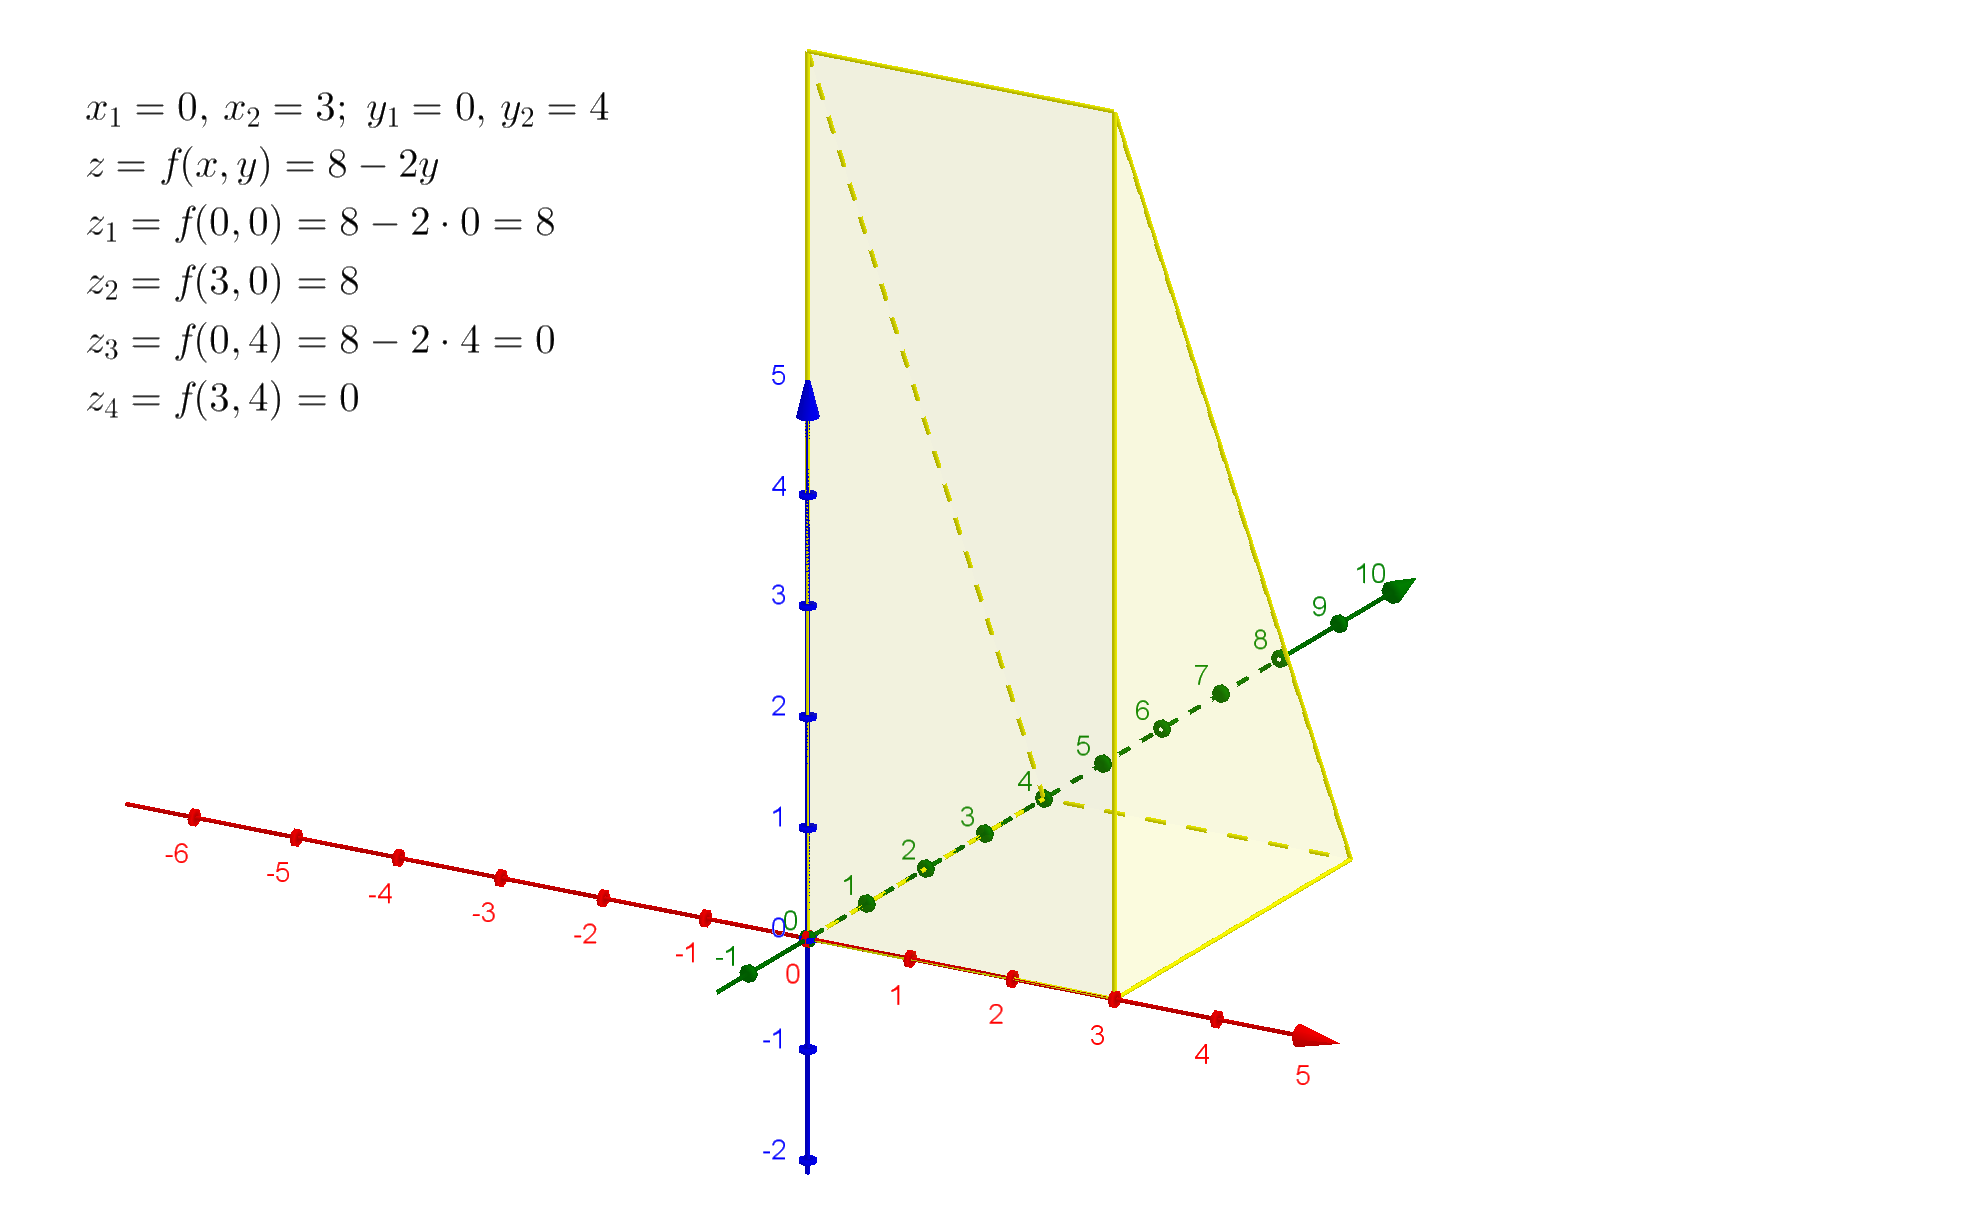
\includegraphics[width=\textwidth]{v01_a03_e02.png}
		\caption{Integrais duplas - Aula 3 - Exercício II}
		\label{v01_a03_e02}
	\end{figure}	
	
	$z = 8 - 2y;\; da = dz = dx dy$\newline\newline
	$v = \integral_0^3 \integral_0^4 z\,dz = \integral_0^3 \integral_0^4(8 - 2y)dx dy = \integral_0^3 dx \integral_0^4(8 - 2y) dy = \integral_0^3 dx \left(8\integral_0^4 dy - 2\integral_0^4 y\,dy\right) = \integral_0^3 dx\, 2\left(4\integral_0^4 dy - \integral_0^4 y\,dy\right) = 2\integral_0^3 dx \left[4y - \dfrac{y^2}{2}\right]_0^4 = 2\integral_0^3 dx \left[\dfrac{8y - y^2}{2}\right]_0^4 = \overstrike{2}\integral_0^3 dx\, \dfrac{1}{\overstrike{2}}[y(8 - y)]_0^4 = \integral_0^3 dx[4(8 - 4) \overstrike{- 0(8 - 0)}] = 16\integral_0^3 dx = 16[x]_0^3 = 16[3 - 0] = 48$
\end{enumerate}		
		\section{Invertendo a ordem de integração - Aula 4}
			\begin{enumerate}
	\item Exercício
	
	\begin{equation*}
		z = f(x, y) = y\e^x;\; dz = dx dy	
	\end{equation*}
	\begin{align*}
		v = \int_2^4 \int_1^9 z\, dz = \int_2^4 \int_1^9 y\e^x\, dy dx = \int_2^4 \e^x\, dx \int_1^9 y\, dy = \int_2^4 \e^x\, dx \left[\dfrac{y^2}{2}\right]_1^9 =\\ \int_2^4 \e^x\, dx \dfrac{1}{2}\left[y^2\right]_1^9 = \dfrac{1}{2}\int_2^4 \e^x\, dx \left[9^2 - 1^2\right] = 40\int_2^4 \e^x\, dx = 40\left[\e^x\right]_2^4 = 40\left[\e^4 - \e^2\right] =\\ 40e^2\left(e^2 - 1\right)	
	\end{align*}
	
	\item Exercício
	
	\begin{equation*}
		z = f(x,y) = x^2y^3;\; dz = dx dy
	\end{equation*}
	
	\begin{figure}[htb]
		\caption{Integrais duplas - Aula 4 - Exercício II}
		\label{v04_a04_e02}
		\centering
		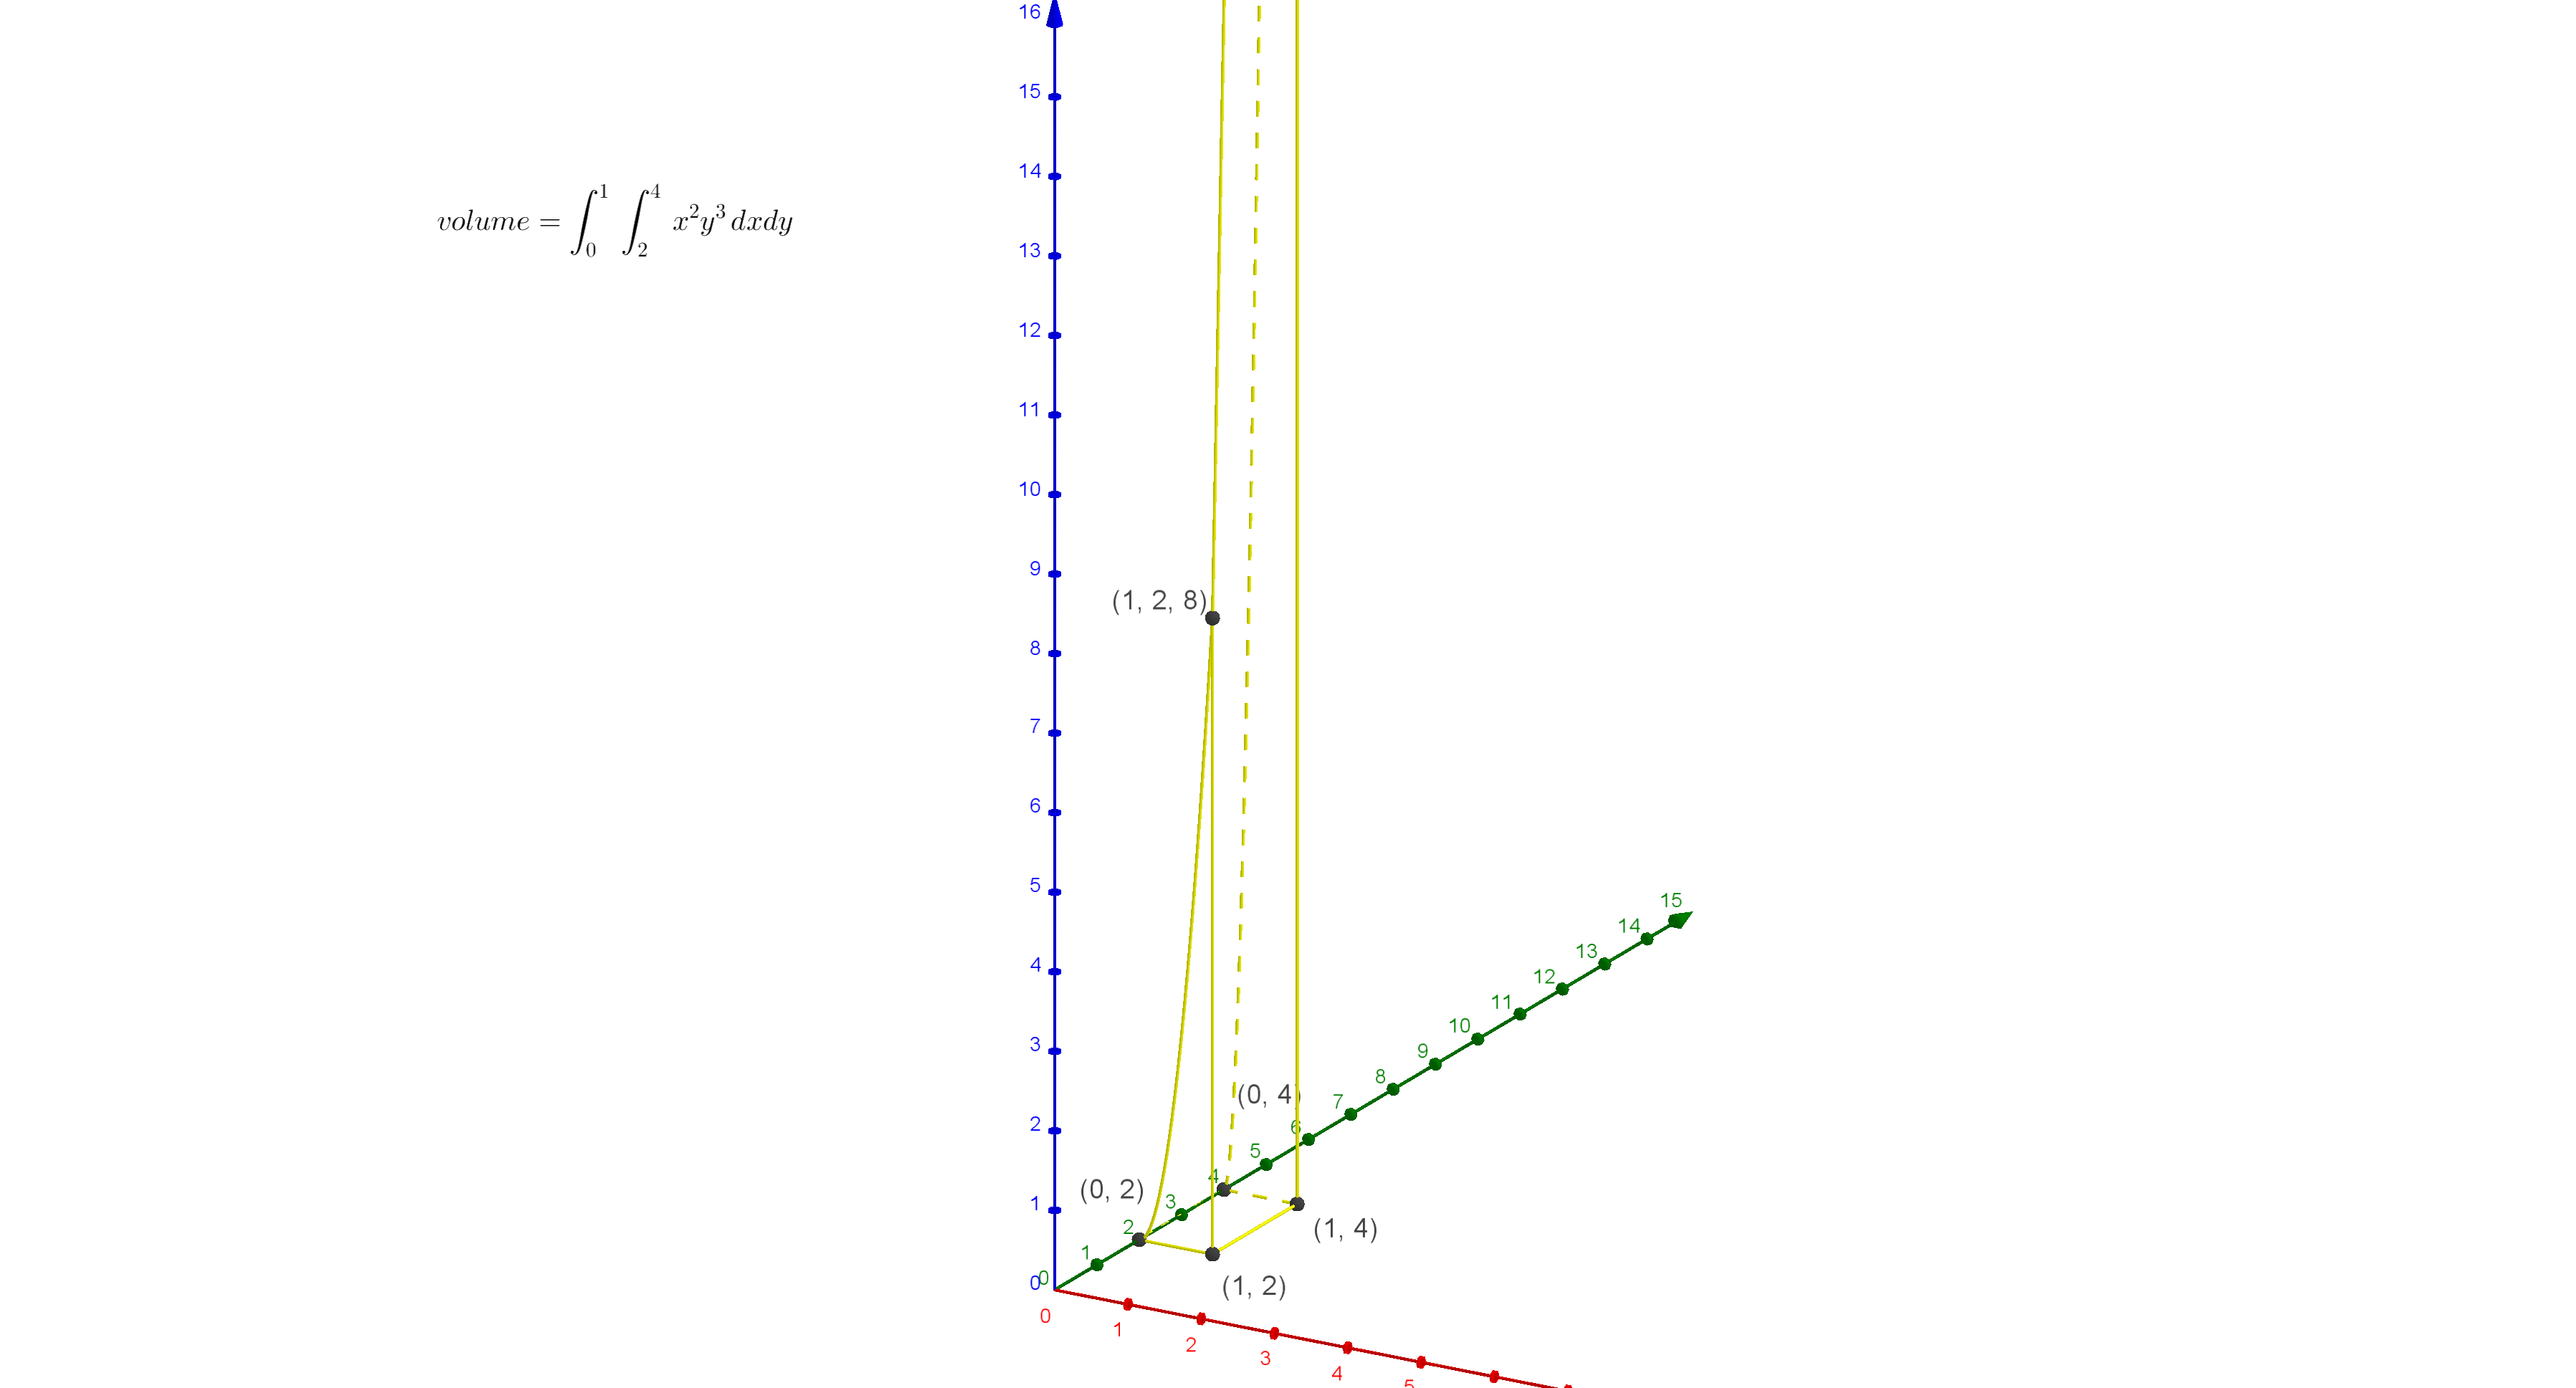
\includegraphics[width=0.5\textwidth]{v04_a04_e02.png}		
	\end{figure}
	
	\begin{align*}
		v = \int_0^1 \int_2^4 z\, dz = \int_0^1 \int_2^4 x^2y^3\, dx dy = \int_0^1 x^2\, dx \int_2^4 y^3\, dy = \int_0^1 x^2\, dx \left[\dfrac{y^4}{4}\right]_2^4 =\\ \dfrac{1}{4}\int_0^1 x^2\, dx \left[y^4\right]_2^4 = \dfrac{1}{4}\int_0^1 x^2\, dx \left[4^4 - 2^4\right] = \dfrac{1}{4}\int_0^1 x^2\, dx \left[2^8 - 2^4\right] =\\ \dfrac{1}{4}\int_0^1 x^2\, dx \left[2^4\left(2^4 - 1\right)\right] = \dfrac{1}{4}\int_0^1 x^2\, dx \left[16 \cdot 15\right] = 60\int_0^1 x^2\, dx = 60 \left[\dfrac{x^3}{3}\right]_0^1 = 20 \left[x^3\right]_0^1 =\\ 20 \left[1^3 - 0^3\right] = 20 \cdot 1 =  20
	\end{align*}
	
	\item Exercício
	
	\begin{equation*}
		\iint_R (x + 2y) da
	\end{equation*}
	
	$R$ = Região limitada pela parábola $y = x^2 + 1$ e as retas $x = -1$ e $x = 2$.
	
	\begin{equation*}
		z = f(x,y) = x + 2y;\; da = dz = dx dy
	\end{equation*}
	
	\begin{figure}[htb]
		\caption{Integrais duplas - Aula 4 - Exercício III}
		\label{v04_a04_e03}
		\centering
		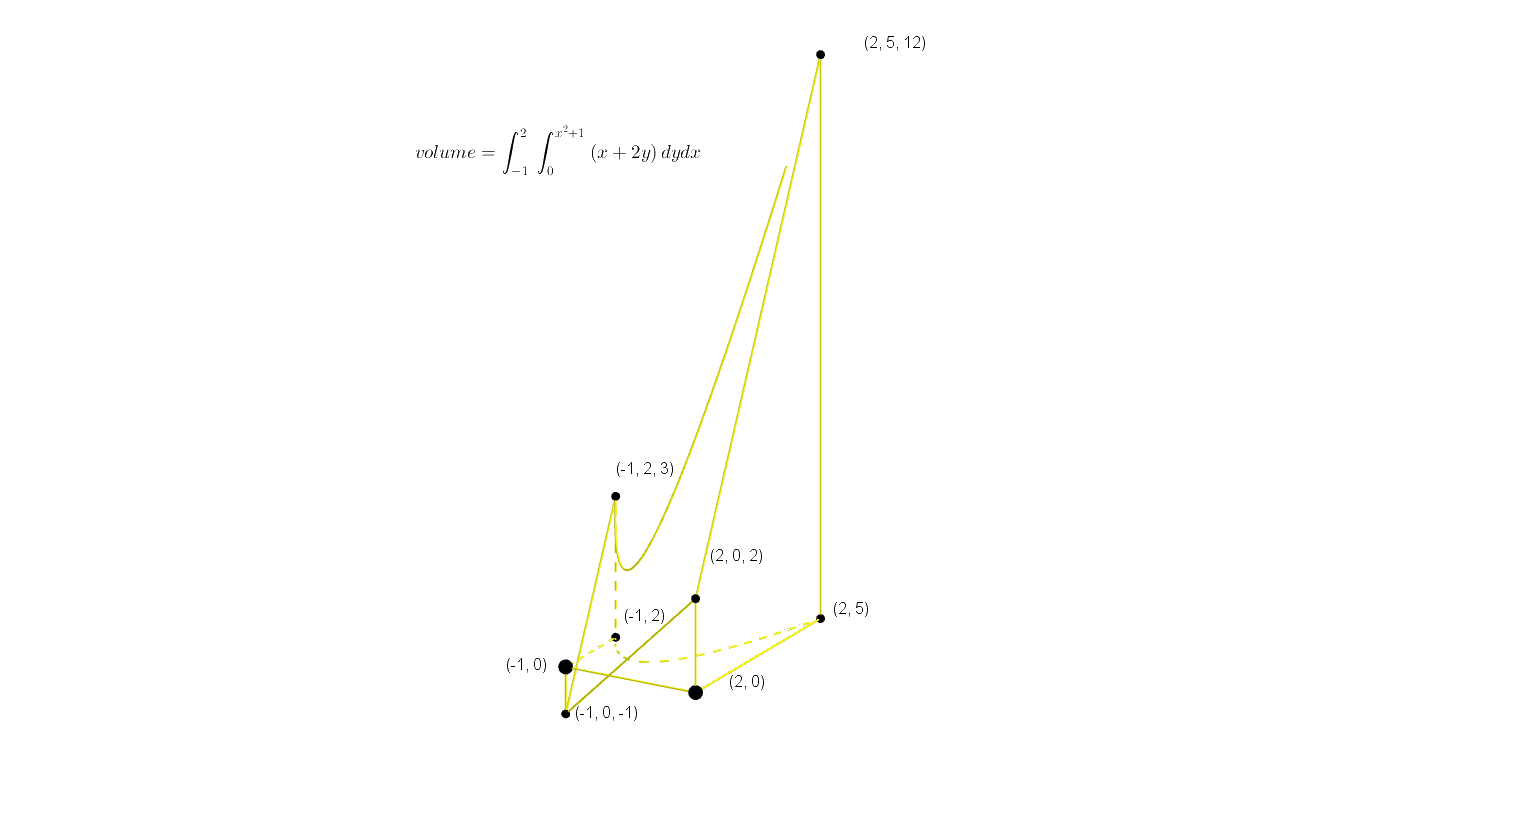
\includegraphics[width=0.5\textwidth]{v04_a04_e03.png}		
	\end{figure}
	
	\begin{align*}
		v = \int_{-1}^2 \int_0^{x^2 + 1} z\, dz = \int_{-1}^2 \int_0^{x^2 + 1} (x + 2y) dx dy =\\ \int_{-1}^2 dx \int_0^{x^2 + 1} (x + 2y) dy = \int_{-1}^2 dx \left(x\int_0^{x^2 + 1} dy + 2\int_0^{x^2 + 1} y\, dy\right) =\\ \int_{-1}^2 dx \left[xy + \overstrike{2}\dfrac{y^2}{\overstrike{2}}\right]_0^{x^2 + 1} = \int_{-1}^2 dx \left[y(x + y)\right]_0^{x^2 + 1} =\\ \int_{-1}^2 dx \left[\left(x^2 + 1\right)\left[x + \left(x^2 + 1\right)\right] \overstrike{- 0(x + 0)}\right] = \int_{-1}^2 dx \left[\left(x^2 + 1\right)\left(x^2 + x + 1\right)\right] =\\ \int_{-1}^2 dx \left(x^4 + x^3 + 2x^2 + x + 1\right) =\\ \int_{-1}^2 x^4\, dx + \int_{-1}^2 x^3\, dx + 2\int_{-1}^2 x^2\, dx + \int_{-1}^2 x\, dx + \int_{-1}^2 dx =\\ \left[\dfrac{x^5}{5} + \dfrac{x^4}{4} + 2\dfrac{x^3}{3} + \dfrac{x^2}{2} + x\right]_{-1}^2 = \left[\dfrac{12x^5 + 15x^4 + 40x^3 + 30x^2 + 60x}{60}\right]_{-1}^2 =\\ \dfrac{1}{60}\left[x\left(12x^4 + 15x^3 + 40x^2 + 30x + 60\right)\right]_{-1}^2 =\\ \dfrac{1}{60}\left[2\left(12\cdot2^4 + 15\cdot2^3 + 40\cdot2^2 + 30\cdot2 + 60\right) \right.\\\left.- (-1)\left(12(-1)^4 + 15(-1)^3 + 40(-1)^2 + 30(-1) + 60\right)\right] =\\ \dfrac{1}{60} [2(192 + 120 + 160 + 60 + 60) + (12 - 15 + 40 - 30 + 60)] = \dfrac{1}{60} (1184 + 67) =\\ \dfrac{1251}{60} = \frac{417}{20} = 20,85
	\end{align*}
\end{enumerate}		
		\section{Cálculo de integrais duplas ou iteradas}
			\subsection{Aula 5}
				\begin{enumerate}
	\item Exercício
	
	\begin{equation*}
		f(x,y) = x^3;\; 0 \leq x \leq 2;\; x^2 \leq y \leq 4	
	\end{equation*}
	\begin{equation*}
		\iint_R f(x, y) dy dx
	\end{equation*}
	
	\begin{figure}[htb]
		\caption{Integrais duplas - Aula 5 - Exercício I}
		\label{v05_a05_e01}
		\centering
		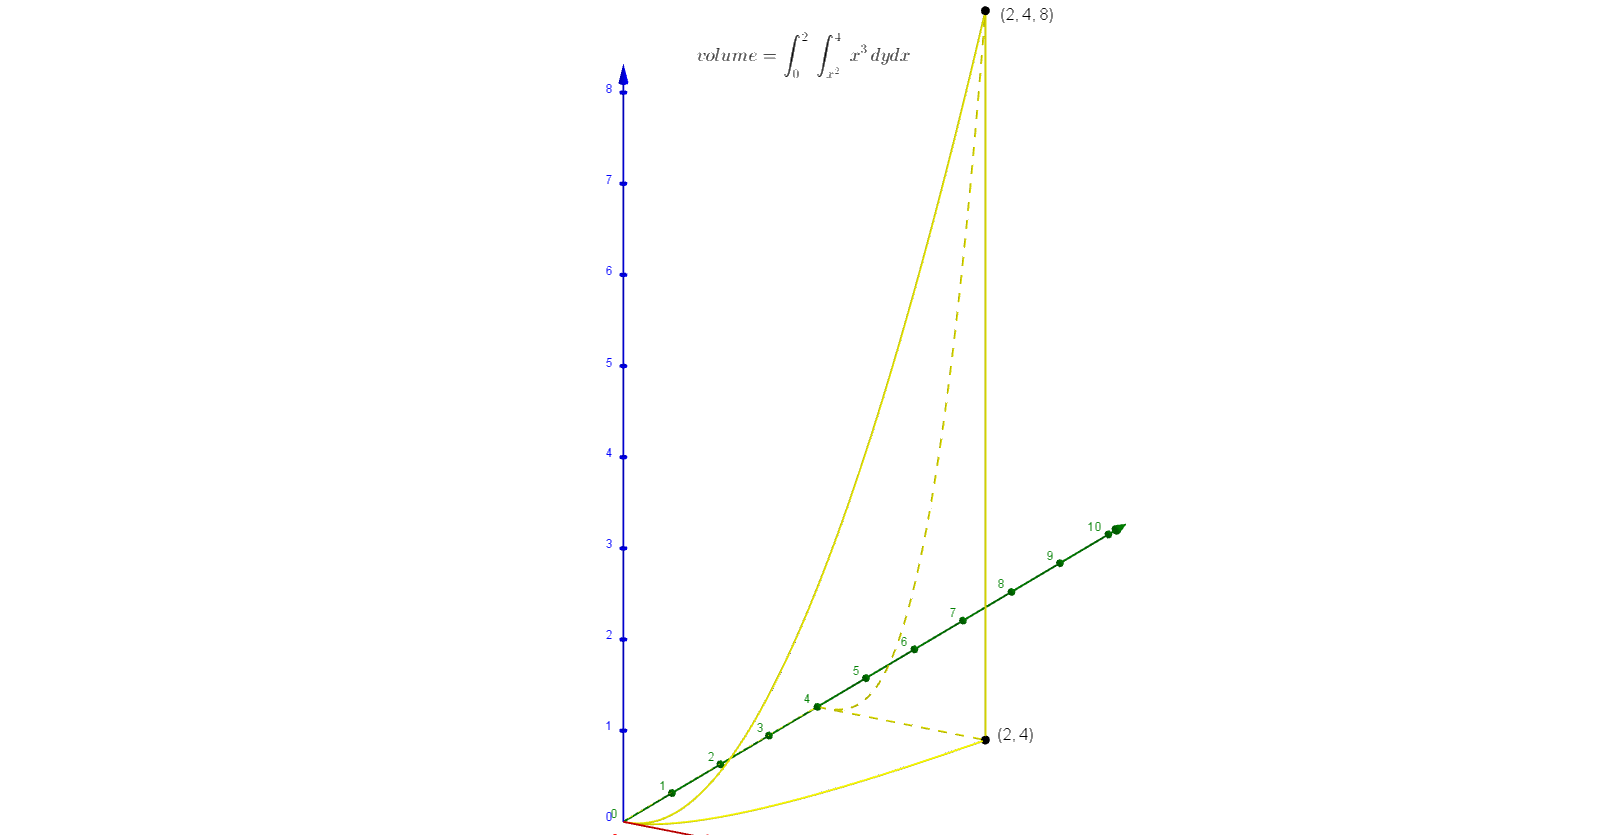
\includegraphics[width=0.5\textwidth]{v05_a05_e01.png}		
	\end{figure}
	
	\begin{gather*}
		v = \int_0^2 \int_{x^2}^4 x^3\, dy dx = \int_0^2 x^3\, dx \int_{x^2}^4 dy = \int_0^2 x^3\, dx\, [y]_{x^2}^4 = \int_0^2 x^3\, dx\, \left[4 - x^2\right] =\\ 4\int_0^2 x^3\, dx - \int_0^2 x^5\, dx = \left[\overstrike{4}\dfrac{x^4}{\overstrike{4}} - \frac{x^6}{6}\right]_0^2 = \left[\dfrac{6x^4 - x^6}{6}\right]_0^2 = \frac{1}{6}\left[x^4\left(6 - x^2\right)\right]_0^2 =\\ \frac{1}{6}\left[2^4\left(6 - 2^2\right) - \overstrike{0^4\left(6 - 0^2\right)}\right] = \dfrac{1}{6}(16\cdot2) = \dfrac{32}{6} = \dfrac{16}{3} = 5,2
	\end{gather*}
	
	\item Exercício
	
	\begin{equation*}
		f(x,y) = x^2y;\; 1 \leq x \leq 3;\; x \leq y \leq 2x + 1
	\end{equation*}
	\begin{equation*}
		\iint_R f(x, y) dy dx
	\end{equation*}
	
	\begin{figure}[htb]
		\caption{Integrais duplas - Aula 5 - Exercício II}
		\label{v05_a05_e02}
		\centering
		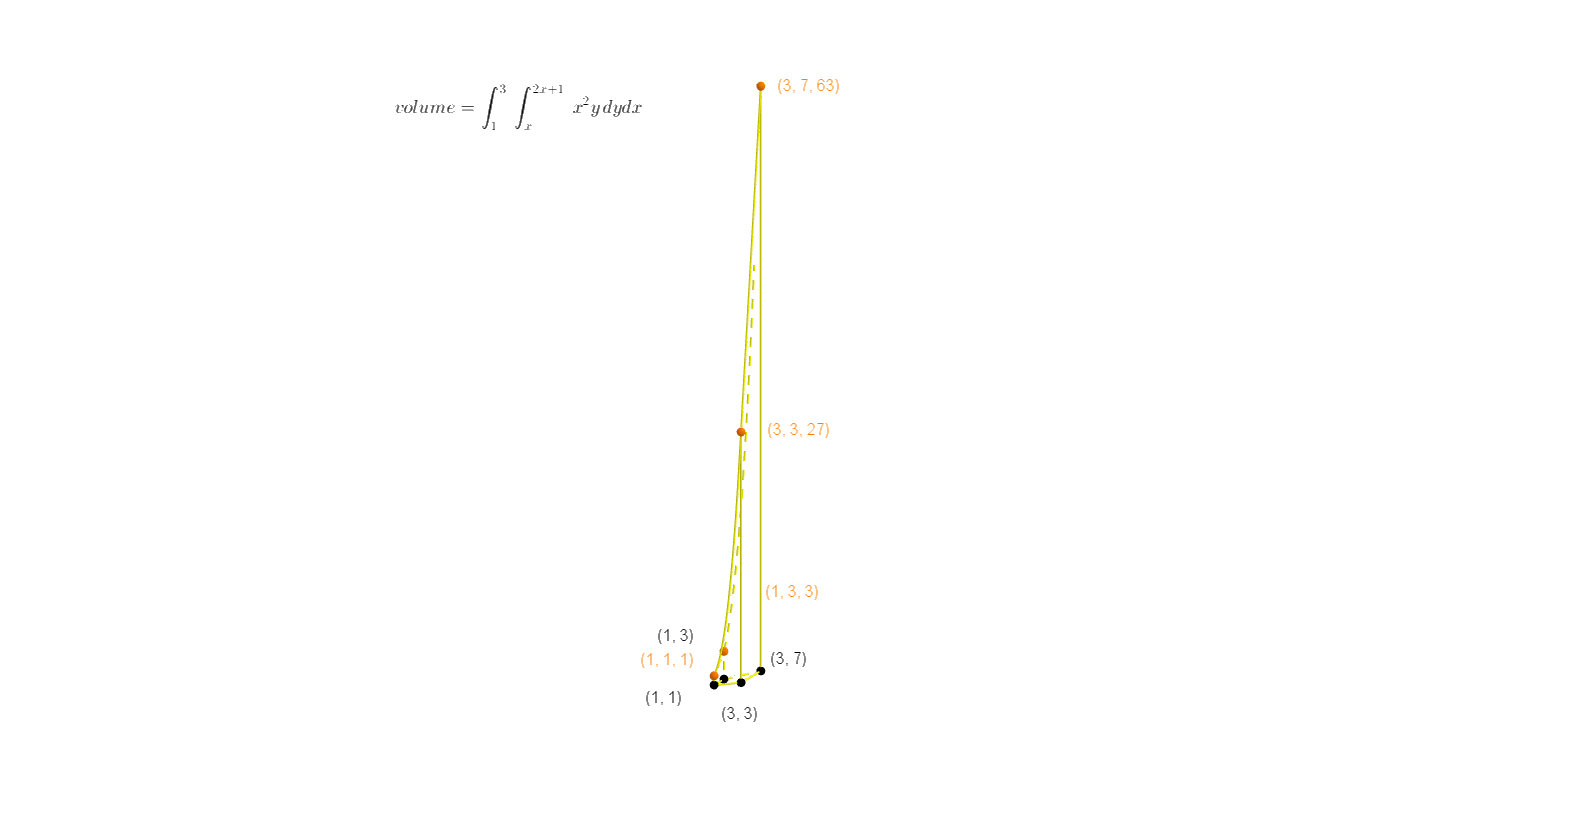
\includegraphics[width=0.5\textwidth]{v05_a05_e02.png}		
	\end{figure}
	
	\begin{gather*}
		v = \int_1^3 \int_x^{2x + 1} x^2y\, dy dx = \int_1^3 x^2\, dx \int_x^{2x + 1} y\, dy =  \int_1^3 x^2\, dx \left[\dfrac{y^2}{2}\right]_x^{2x + 1} =\\  \int_1^3 x^2\, dx \dfrac{1}{2}\left[(2x + 1)^2 - (x)^2\right] = \dfrac{1}{2}\int_1^3 x^2\, dx \left(3x^2 + 4x + 1\right) =\\ \dfrac{3}{2}\int_1^3 x^4\, dx + 2\int_1^3 x^3\, dx + \dfrac{1}{2}\int_1^3 x^2\, dx = \left[\dfrac{3}{2}\dfrac{x^5}{5} + 2\frac{x^4}{4} + \dfrac{1}{2}\dfrac{x^3}{3}\right]_1^3 = \left[\dfrac{3x^5}{10} + \dfrac{x^4}{2} + \frac{x^3}{6}\right]_1^3 =\\ \left[\dfrac{18x^5 + 30x^4 + 10x^3}{60}\right]_1^3 = \left[\dfrac{2x^3\left(9x^2 + 15x + 5\right)}{60}\right]_1^3 =\\ \dfrac{1}{30}\left[x^3\left(9x^2 + 15x + 5\right)\right]_1^3 = \dfrac{1}{30}\left[3^3\left(9\cdot3^2 + 15\cdot3 + 5\right) - 1^3\left(9\cdot1^2 + 15\cdot1 + 5\right)\right] =\\ \dfrac{1}{30}\left[27(81 + 45 + 5) - (9 + 15 + 5)\right] = \dfrac{1}{30}\left[27\cdot131 - 29\right] = \frac{3508}{30} = 116,9\overline{3}	
	\end{gather*}
\end{enumerate}		
			\subsection{Aula 6}
				\begin{enumerate}
	\item Exercício
	
	$f(x,y) = 1;\; 0 \leq x \leq 1;\; 1 \leq y \leq \e^x$\newline
	$\iintegral_R f(x, y) dy dx$\newline\newline
	$v = \integral_0^1 \integral_1^{\e^x} dy dx = \integral_0^1 dx\, [y]_1^{\e^x} = \integral_0^1 dx\, \left(\e^x - 1\right) = \left[\e^x - x\right]_0^1 = \e^1 - 1 - \left(\e^0 - 0\right) = \e - 1 - 1 = \e - 2$\newline
	
	\item Exercício
	
	$f(x,y) = x;\; 0 \leq x \leq 1;\; 1 \leq y \leq \e^{x^2}$\newline
	$\iintegral_R f(x, y) dy dx$\newline\newline
	$v = \integral_0^1 \integral_1^{\e^{x^2}} x\,	dx dy = \integral_0^1 x\,	dx \integral_1^{\e^{x^2}} dy = \integral_0^1 x\,	dx\, [y]_1^{\e^{x^2}} = \integral_0^1 x\,	dx\, \left(\e^{x^2} - 1\right) = \integral_0^1 x\e^{x^2}\,	dx - \integral_0^1 x\,	dx = \integral_0^1 \e^u\, \dfrac{du}{2} - \integral_0^1 x\,	dx = \dfrac{1}{2}\integral_0^1 \e^u\, du - \integral_0^1 x\,	dx = \left[\dfrac{1}{2}e^u - \dfrac{x^2}{2}\right]_0^1 = \left[\dfrac{e^{x^2} - x^2}{2}\right]_0^1 = \dfrac{1}{2} \left[e^{x^2} - x^2\right]_0^1 = \dfrac{1}{2} \left[e^{1^2} - 1^2 - \left(e^{0^2} - 0^2\right)\right] = \dfrac{1}{2}(\e - 1 - 1) = \dfrac{\e - 2}{2}$\newline\newline
	$u = x^2 ;\; \dfrac{du}{2} = x\, dx$
	
	\item Exercício
	
	$f(x,y) = 2xy;\; 0 \leq y \leq 1;\; y^2 \leq x \leq y$\newline
	$\iintegral_R f(x, y) dx dy$\newline\newline
	$v = \integral_0^1 \integral_{y^2}^y 2xy\, dx dy = 2\integral_0^1 y\, dy \integral_{y^2}^y x\, dx = 2\integral_0^1 y\, dy\, \left[\dfrac{x^2}{2}\right]_{y^2}^y = \overstrike{2}\integral_0^1 y\, dy\, \dfrac{1}{\overstrike{2}}\left[x^2\right]_{y^2}^y = \integral_0^1 y\, dy\, \left(y^2 - y^4\right) = \integral_0^1 \left(y^3 - y^5\right) dy = \left[\frac{y^4}{4} - \frac{y^6}{6}\right]_0^1 = \left[\dfrac{6y^4 - 4y^6}{24}\right]_0^1 = \left[\dfrac{2y^4\left(3 - 2y^2\right)}{24}\right]_0^1 = \dfrac{1}{12}\left[1^4\left(3 - 2\cdot1^2\right) \overstrike{- 0^4\left(3 - 2\cdot0^2\right)}\right] = \dfrac{1}{12} = 0,08\overline{3}$
\end{enumerate}		
			\subsection{Aula 7}
				\begin{enumerate}
	\item Exercício
	
	\begin{equation*}
		f(x,y) = \dfrac{1}{x + y};\; 1 \leq y \leq \e;\; 0 \leq x \leq y	
	\end{equation*}
	\begin{equation*}
		\iint_R f(x, y) dx dy
	\end{equation*}
	\begin{gather*}
		v = \int_1^{\e} \int_0^y \dfrac{1}{x + y}\, dx dy = \int_1^{\e} dy \int_0^y (x + y)^{-1}\, dx = \int_1^{\e} dy \int_0^y u^{-1}\, du =\\ \int_1^{\e} dy \int_0^y\, \left[\ln |u|\right]_0^y = \int_1^{\e} dy \int_0^y\, \left[\ln |x + y|\right]_0^y = \int_1^{\e} dy \int_0^y\, \left(\ln |y + y| - \ln |0 + y|\right) =\\ \int_1^{\e} dy \int_0^y\, \left(\ln |2y| - \ln |y|\right) = \int_1^{\e} dy \int_0^y\, \left(\ln |2| \overstrike{+ \ln |y| - \ln |y|}\right) = \ln |2|\int_1^{\e} dy =\\ \ln |2|[y]_1^{\e} = \ln |2|(\e - 1)
	\end{gather*}
	\begin{equation*}
		u = x + y;\; du = (1 + 0)dx = dx
	\end{equation*}
\end{enumerate}
		
		%\section{Cálculo de área - Aula 8}
		
		%\section{Cálculo de volume}
			%\subsection{Aula 9}
		
			%\subsection{Aula 10}		
	
		%\section{Coordenadas polares}		
			%\subsection{Aula 1}
			
			%\subsection{Aula 2}
			
			%\subsection{Aula 3}
			
	%\part{Integrais triplas}
	
		%\section{Introdução - Aula 1}
		
		%\section{Cálculo de integrais triplas - Aula 2}
		
		%\section{Cálculo do volume de um sólido - Aula 3}
		
		%\section{Esboço de um sólido - Aula 4}
	
		%\section{Coordenadas esféricas}
			%\subsection{Aula 1}
			
			%\subsection{Aula 2}
			
			%\subsection{Aula 3}
			
			%\subsection{Aula 4}
			
			%\subsection[Aula 5]{Cálculo de massa com coordenadas esféricas - Aula 5}
			
			%\subsection{Aula 6}
			
			%\subsection{Aula 7}
	
		%\section{Coordenadas cilíndricas}
			%\subsection{Aula 1}
			
			%\subsection{Aula 2}
			
			%\subsection{Aula 3}
			
			%\subsection{Aula 4}
			
			%\subsection{Aula 5}
			
			%\subsection{Aula 6}
			
			%\subsection{Aula 7}
			
			%\subsection{Aula 8}
\end{document}
